% Chapter 6: Model Graphs page
\chapter{Model Graphs}\label{sec:ch06-graphs}\label{chap:6}

The \ui{Model Graphs} page (navigation group \ui{Analysis}) draws the fitted model of a response, or of
several responses together, as contour plots, surfaces and effect plots. The graphs show what the
equations of Chapter~\ref{chap:5} mean in the factor space: where the response is high or low, how strongly each
factor acts, whether factors interact, and where all requirements are met at the same time.

\section{Controls and common behavior}\label{sec:ch06-controls}

\subsection*{Purpose}
The page answers the question ``what does the model predict, and where?''. It does not fit anything
itself: it uses the model selected on the \ui{RSM Analysis} page, or the ANN model when the response is
switched to ANN.

\subsection*{How to use}
\begin{enumerate}
  \item Choose the response in \ui{Response:} and the graph in \ui{Type:}.
  \item Choose the factors on the axes (the axis selectors and their labels depend on the graph type,
        Table~\ref{tab:ch06-controls}). If two selectors hold the same factor, the program changes one of
        them automatically.
  \item Set the values of the factors that are not on an axis in the group \ui{Other Factor Values}. The
        graph is a \emph{slice} through the factor space at these values.
  \item Use the plot toolbar to zoom, pan, save the image, copy or export the data
        (Section~\ref{sec:ch06-export}). 3D graphs can be rotated with the mouse.
\end{enumerate}

\begin{table}[htbp]\centering\small
\caption{Controls of the Model Graphs page.}\label{tab:ch06-controls}
\begin{tabularx}{\linewidth}{@{}>{\raggedright\arraybackslash}p{2.6cm} >{\raggedright\arraybackslash}p{4.4cm} >{\raggedright\arraybackslash}p{1.6cm} X@{}}
\toprule
Control & Values & Default & Meaning \\
\midrule
\ui{Response:} & each response & first & Response to plot (not used by Overlay and Desirability, which use all responses with a goal). \\
\ui{Type:} & see Section~\ref{sec:ch06-types} & first type & Graph type. \\
Axis selectors & \ui{X axis:}, \ui{Y axis:}; Interaction: \ui{X axis:}, \ui{Lines (second factor):}; Cube: \ui{X axis:}, \ui{Y axis:}, \ui{Depth axis:}; mixtures: \ui{Top vertex:}, \ui{Left vertex:}, \ui{Right vertex:} & first factors & Factors on the axes. Contour-type graphs and the cube accept only numeric factors. \\
\ui{Contour lines:} & 4--40 & 12 & Number of contour levels (contour, desirability and POE graphs). \\
\ui{Other Factor Values} & one control per factor not on an axis & see text & Values at which the slice is taken. Title \ui{Other Components (Actual Units)} for mixtures, \ui{Reference Levels} for All Factors and \ui{Reference Point} (one control for every factor) for Perturbation. \\
\bottomrule
\end{tabularx}
\end{table}

\paragraph{Slice controls.} A numeric factor gets a spin box in actual units. Its range runs from the
smaller of the data minimum and the low level to the larger of the data maximum and the high level, so axial
points of a CCD can be reached. The default is the middle of the range, $(\text{low}+\text{high})/2$; for
mixture components it is the design centroid in actual units. The step is 1/20 of the range, with 4
decimals for ranges below 10 and 2 decimals otherwise. A categoric factor gets a list of its levels; the
default is the first level. The values are kept when you change the graph type.

\paragraph{Note below the controls.} Every graph adds ``Red points = design runs in this slice (number =
replicate count).'' For process designs the contour, surface, overlay and desirability graphs add ``Graph
range = levels -1 to +1. Gray area = outside the constraints.'' Mixture designs add ``Mixture graphs are
drawn in pseudo-component space.'' Some types add their own sentence (given in the sections below).

\paragraph{Model source (RSM or ANN).} Each response uses the model chosen for it: RSM by default, or the
ANN when \ui{Use this response's ANN for graphs, optimization, NSGA-II \& prediction} is checked on the
\ui{ANN} page (or \ui{ANN} is chosen in the \ui{Model} column of the \ui{Desirability} page). The response
label then ends in ``[ANN]''. ANN models have no confidence bands, and their POE uses the mean squared error
of the network over all data.

\paragraph{Messages.}
\begin{itemize}
  \item ``This graph needs more numeric factors.'' The type needs more numeric factors than the design has
        (for example a cube plot with two numeric factors).
  \item ``\dots{} Enter response data, then check Analysis.'' No model can be computed yet (the first line
        gives the reason).
  \item ``No criteria yet. Choose response goals and limits on the Desirability page.'' Overlay and
        Desirability need goals; they are set on the \ui{Desirability} page.
  \item ``This slice lies entirely outside the design region. Change the values of the other
        factors/components.'' The slice values violate the bounds or the linear constraints everywhere.
\end{itemize}

\section{The slice grid (theory as implemented)}\label{sec:ch06-grid}

\paragraph{Process designs.} Contour-type graphs evaluate the model on a $60\times60$ grid over the coded
square $[-1,1]^2$ of the two axis factors, with all other factors at the slice values. The axes are labeled
in actual units. Points that violate a linear constraint are outside the feasible region: the region is
drawn grey and the plots are clipped with the exact feasible polygon, computed from the bounds and the
constraints.

\paragraph{Mixture designs.} Ternary graphs evaluate the model on a triangular lattice of resolution 60
over the three chosen components (in pseudo-components), scaled to $1-\sum(\text{other components})$ when
the mixture has more than three components. If less than 20\% of the lattice is feasible, the resolution is
raised to 180. A point with pseudo-components $(a,b,c)$ (top, left, right vertex) is drawn at
$X=c+a/2$, $Y=a\sqrt3/2$. Grid lines of each component are labeled in actual units. When the feasible
region is small, the view zooms in on it, with the note ``Zoomed to the feasible region. Numbers on lines =
component amount (actual units).''; otherwise the vertex amounts are written at the corners.

\paragraph{Design points.} Runs whose coordinates off the axes agree with the slice values within $10^{-3}$
(coded) are drawn as red points; a number next to a point gives the number of replicates at that location.
On contour, overlay, desirability and POE graphs the best desirability solution (the first row of the last
desirability result) is drawn as a yellow star labeled ``Optimum'' when it lies within 0.02 (coded) of the
slice.

\paragraph{Confidence bands.} One-factor, all-factor and interaction graphs show the 95\% confidence
interval of the mean response,
\begin{equation}
  \hat y_0\pm t_{0.975,\,n-p}\sqrt{\text{MSE}\,h_0},\qquad h_0=x_0'(X'X)^{+}x_0,
  \label{eq:ch06-ci}
\end{equation}
computed on the transformed scale and back-transformed. For GLM responses the band is
$g^{-1}(\hat\eta\pm1.96\,\text{se}_\eta)$, for split-plot responses it uses the REML covariance of the
coefficients. No band is drawn when the model has no residual degrees of freedom, or for ANN models.

\section{Graph types}\label{sec:ch06-types}

Process designs offer \ui{2D Contour}, \ui{3D Surface}, \ui{One Factor Effect}, \ui{All Factors},
\ui{Interaction}, \ui{Cube Plot}, \ui{Perturbation}, \ui{Overlay (Graphical Optimization)} and
\ui{Desirability Contour}. Mixture and combined mixture-process designs offer \ui{Ternary Contour},
\ui{3D Ternary Surface}, \ui{Trace (Piepel)}, \ui{Overlay (Graphical Optimization)} and
\ui{Desirability Contour}. Both lists end with \ui{Propagation of Error (POE)} when at least one factor has a
standard deviation $\sigma>0$ (Section~\ref{sec:ch06-poe}). Table~\ref{tab:ch06-axes} summarizes the axes.

\begin{table}[htbp]\centering\small
\caption{Axes needed by each graph type.}\label{tab:ch06-axes}
\begin{tabular}{@{}lcc@{}}
\toprule
Graph & Axis factors & Numeric only \\
\midrule
2D Contour, 3D Surface, Overlay, Desirability, POE (process) & 2 & yes \\
One Factor Effect & 1 & no \\
Interaction & 2 & no \\
Cube Plot & 3 & yes \\
Perturbation & all numeric factors & yes \\
All Factors & all factors & no \\
Ternary graphs, Overlay, Desirability, POE (mixture) & 3 components & yes \\
Trace (Piepel) & all components & yes \\
\bottomrule
\end{tabular}
\end{table}

The examples in this chapter use the Box-Behnken extraction case, response Yield, with Temperature on the
X axis, Time on the Y axis and Concentration at 2\%, unless stated otherwise.

\subsection{2D Contour}\label{sec:ch06-contour}
\paragraph{Purpose.} Shows the predicted response over two factors as filled contours, to locate the
optimum region and see the shape of the surface (ridge, saddle, maximum).

\paragraph{Output.} Filled contours of $\hat y$ (original units) with the number of levels from
\ui{Contour lines:}, black contour lines labeled with their value, a color bar, the design points of the
slice and the optimum star.

\paragraph{Example.} Figure~\ref{fig:ch06-contour}: Yield rises toward high Temperature and high Time; the
model maximum in this slice is 80.2\% at about 75 °C and 85 min. The center point is labeled ``5'' (five
replicates).

\begin{figure}[htbp]\centering
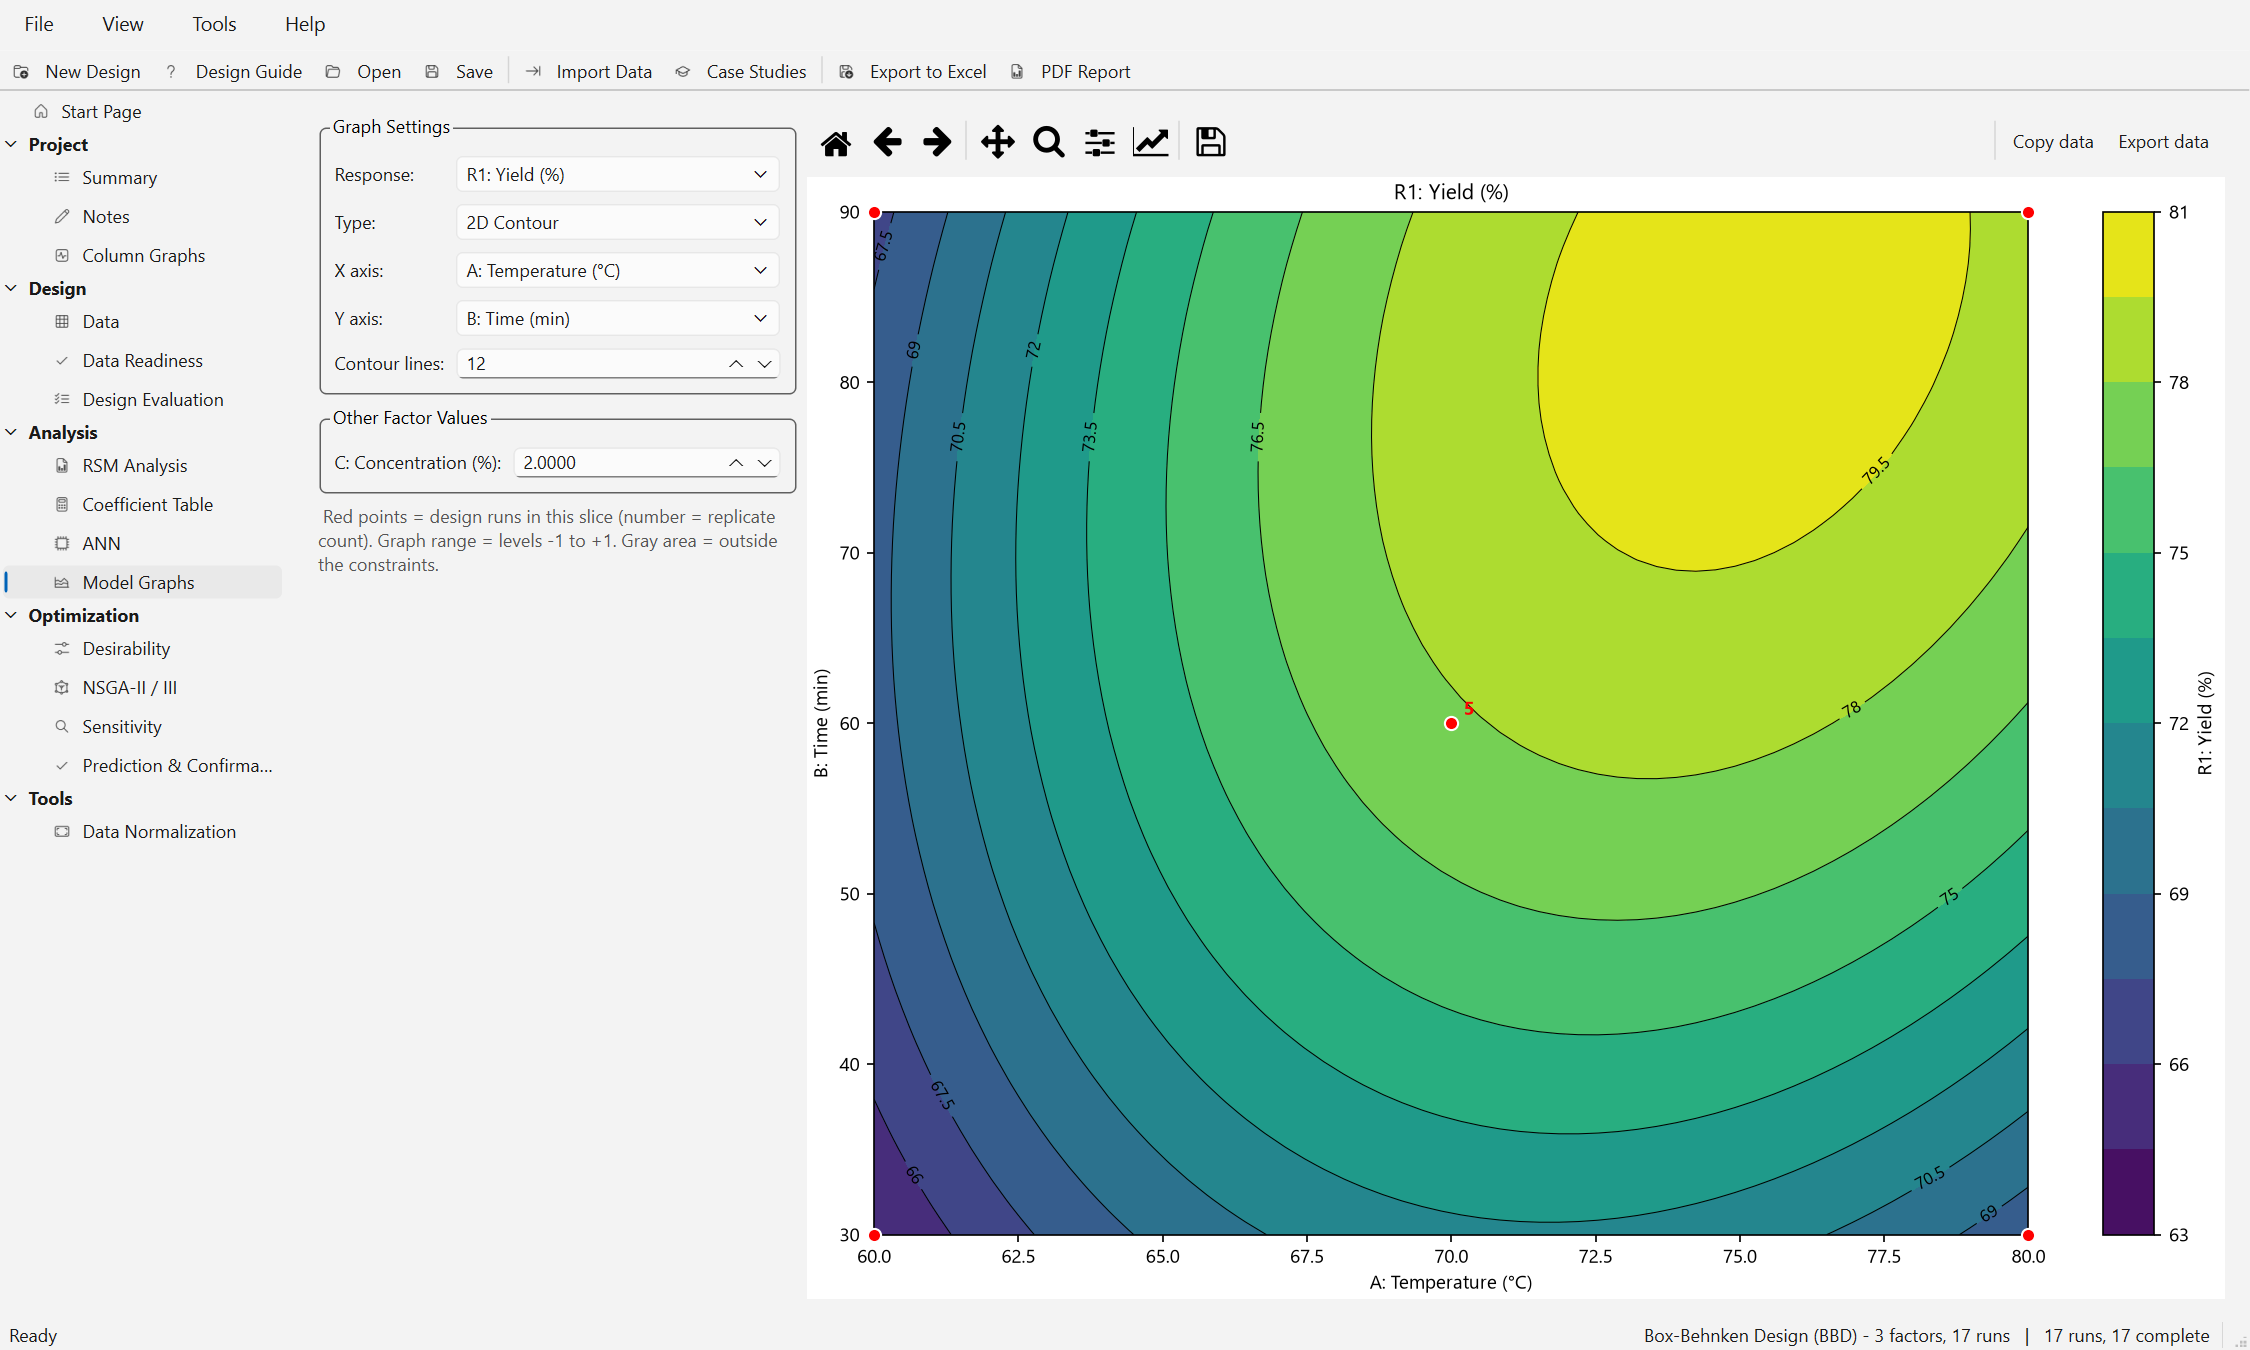
\includegraphics[width=\linewidth]{graph_contour.png}
\caption{2D Contour of Yield (Temperature $\times$ Time, Concentration 2\%) with the design points in the
slice.}
\label{fig:ch06-contour}
\end{figure}

\subsection{3D Surface}\label{sec:ch06-surface}
\paragraph{Purpose.} The same slice as a surface, which makes curvature easy to see.
\paragraph{Output.} A surface of $\hat y$ over the two axis factors (points outside the feasible region are
left out), a color bar, and the observed responses of the runs in the slice as red points, so the distance
between data and surface is visible (Figure~\ref{fig:ch06-surface}).

\begin{figure}[htbp]\centering
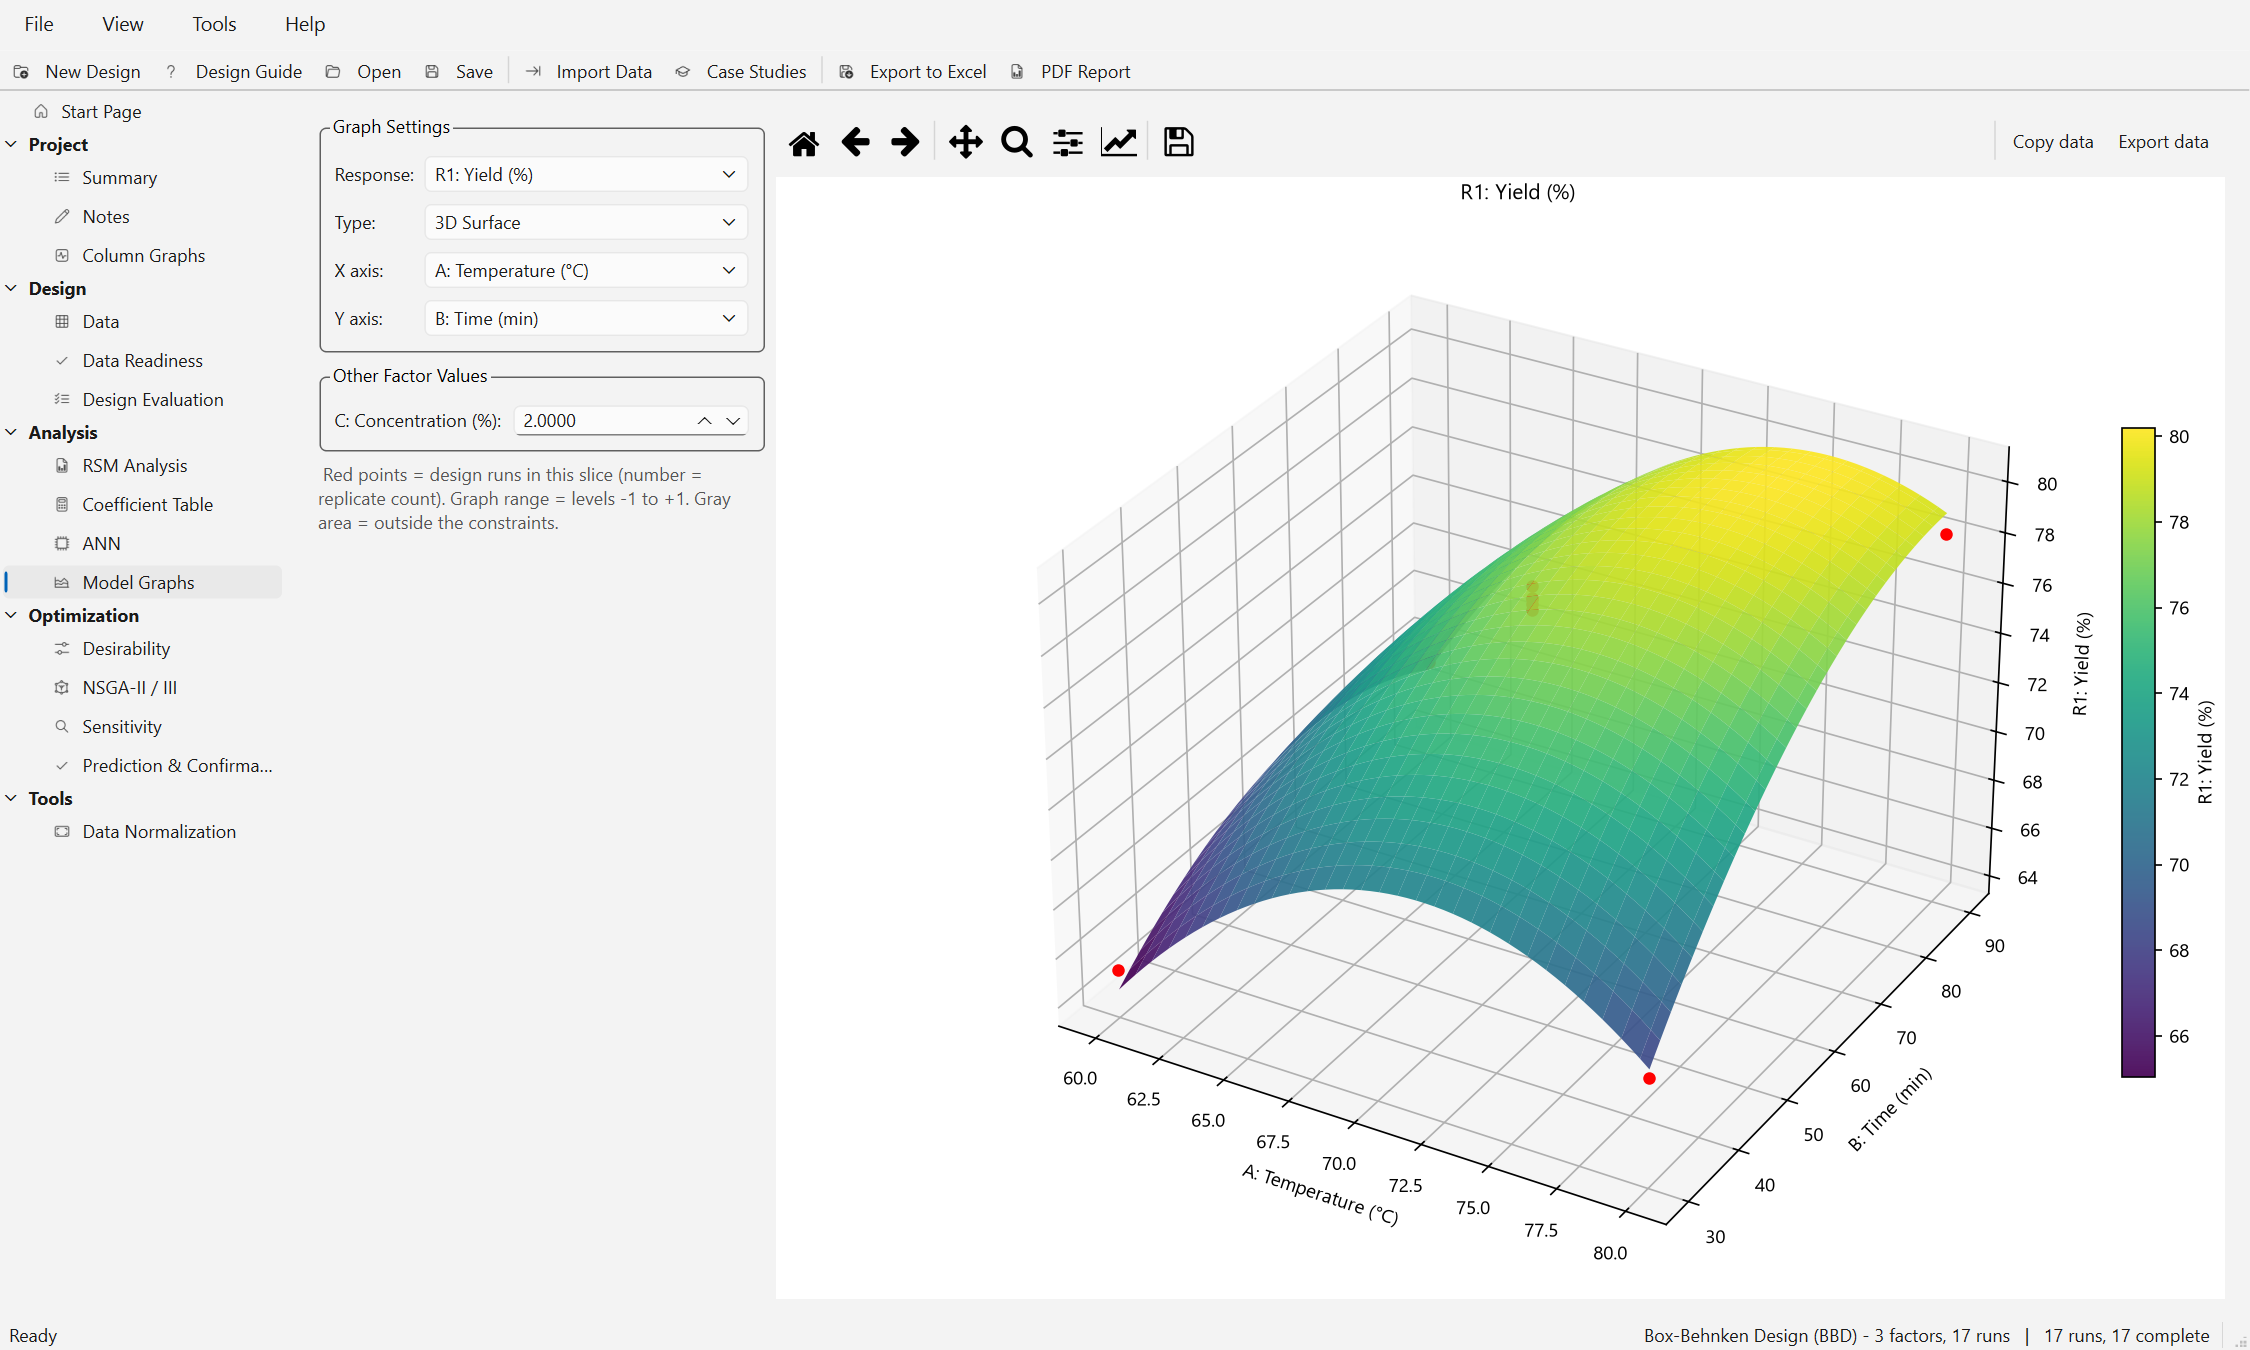
\includegraphics[width=0.85\linewidth]{graph_surface3d.png}
\caption{3D Surface of Yield over Temperature and Time.}
\label{fig:ch06-surface}
\end{figure}

\subsection{One Factor Effect}\label{sec:ch06-oneway}
\paragraph{Purpose.} Shows how the response changes along one factor, with the other factors at the slice
values, and how precisely the model predicts it.
\paragraph{Output.} For a numeric factor: the prediction over the coded range $-1$ to $+1$ (100 points,
axis in actual units) with the 95\% confidence band \eqref{eq:ch06-ci}. For a categoric factor: one point per
level with 95\% error bars. Red points are the runs in the slice. Title ``Effect of \dots''.
\paragraph{Example.} Figure~\ref{fig:ch06-oneway}: Yield against Temperature at Time 60 min and
Concentration 2\% is curved, with a maximum of 78.5\% near 73.6 °C. The five center runs appear at 70 °C.

\begin{figure}[htbp]\centering
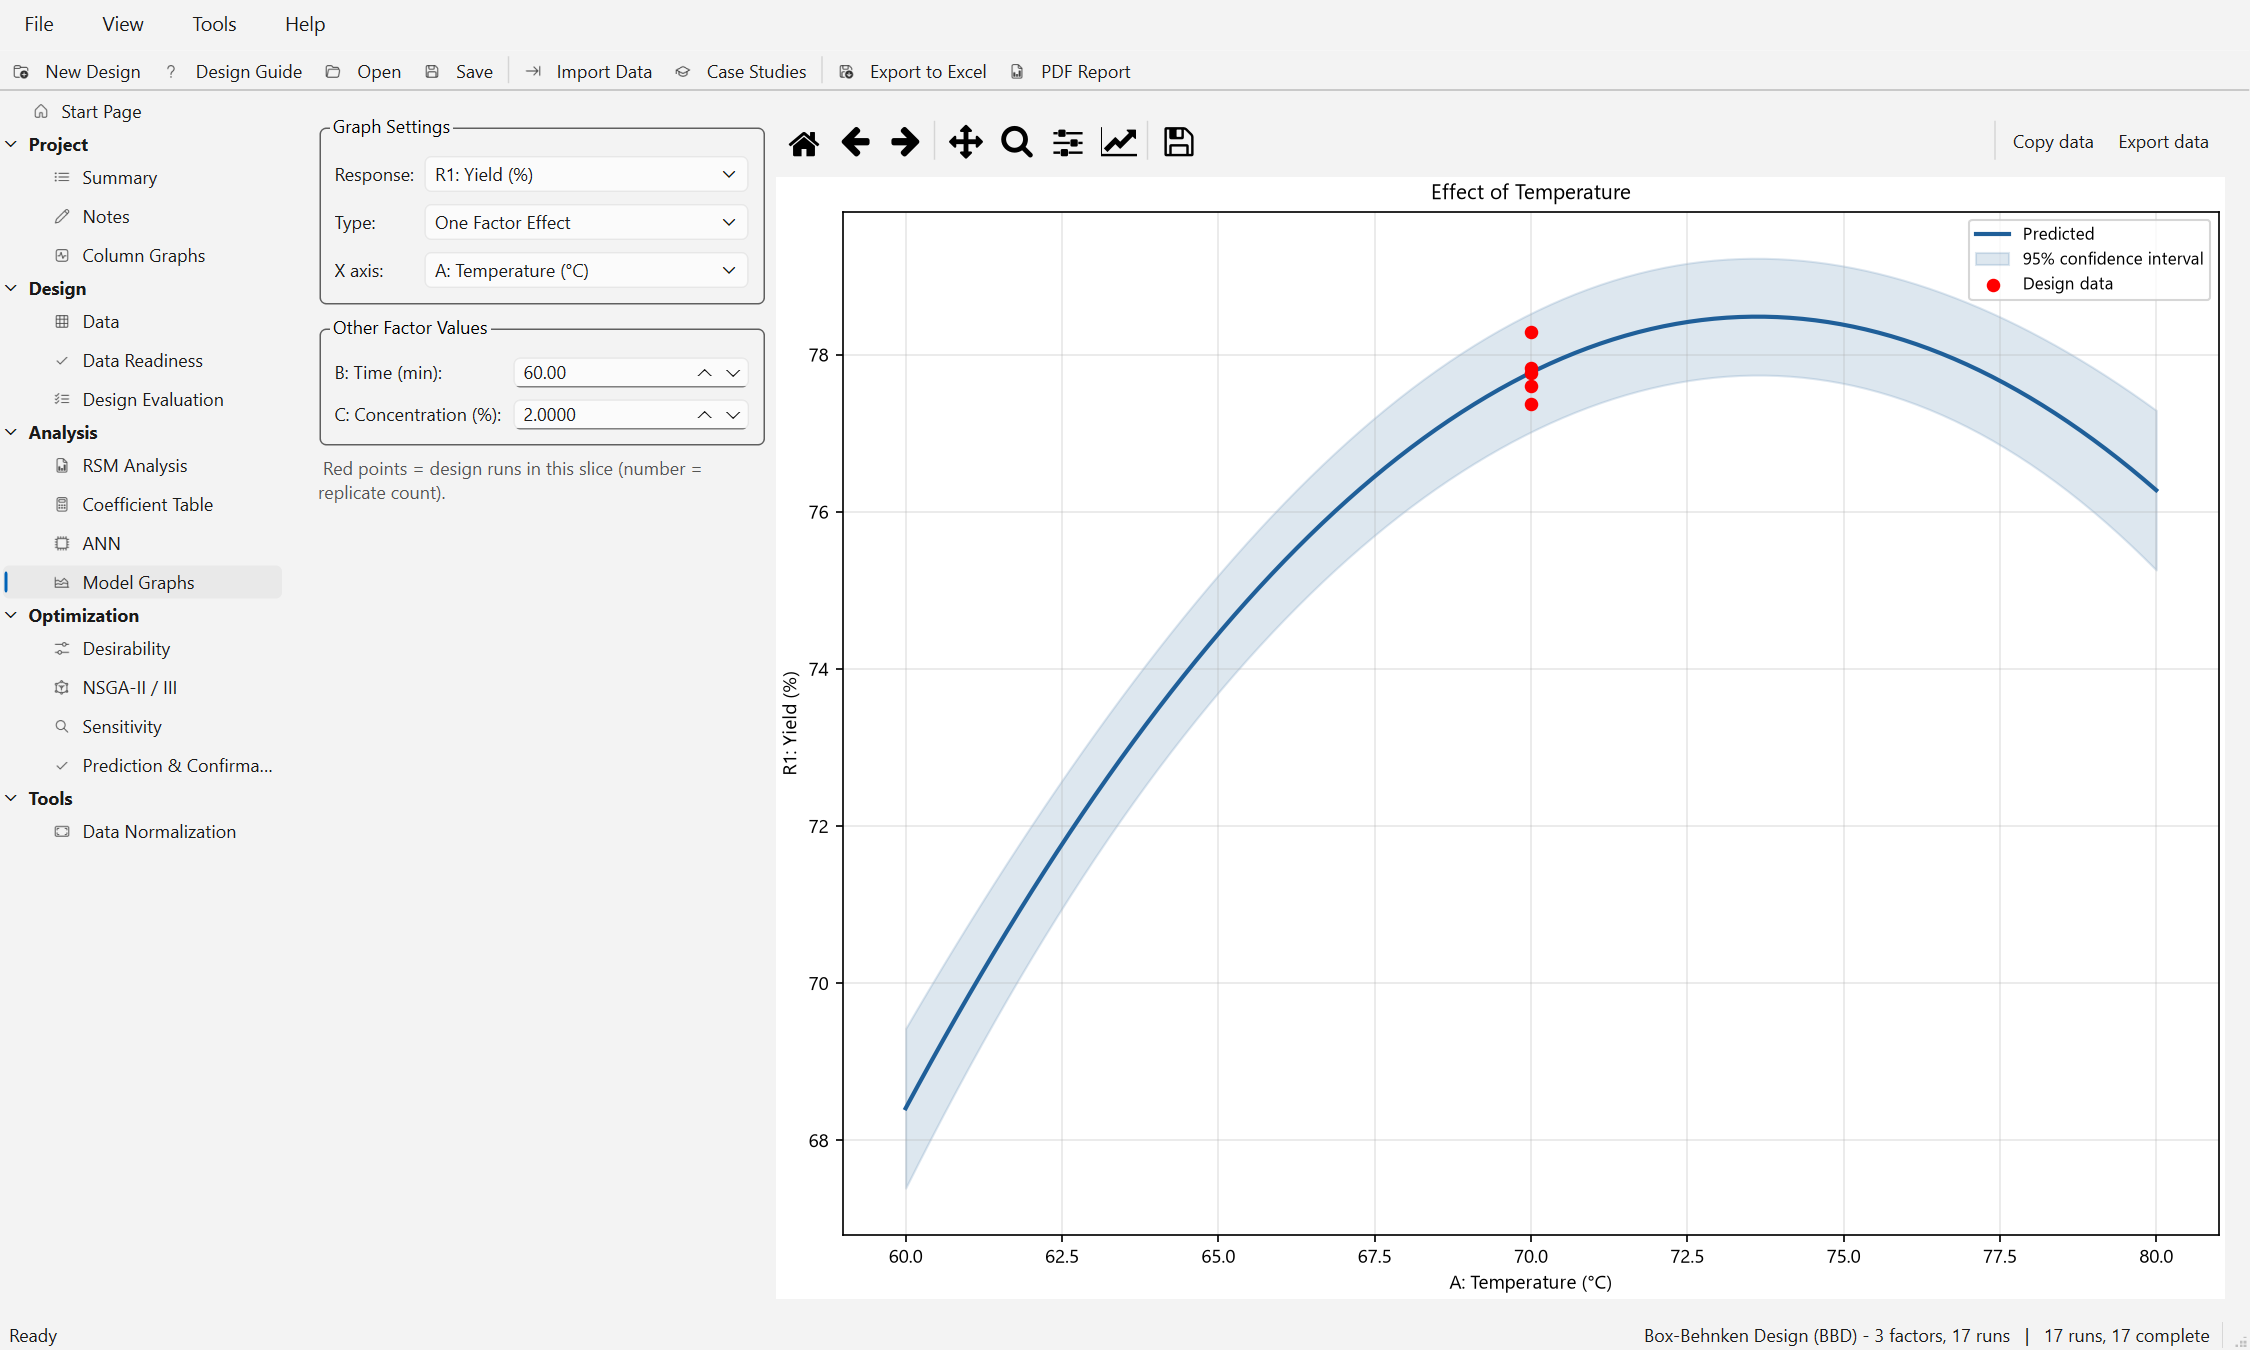
\includegraphics[width=\linewidth]{graph_oneway.png}
\caption{One Factor Effect of Temperature on Yield with the 95\% confidence band.}
\label{fig:ch06-oneway}
\end{figure}

\subsection{All Factors}\label{sec:ch06-allfactors}
\paragraph{Purpose.} One-factor effects of all factors at once, on a shared response axis, so the size of
the effects can be compared directly.
\paragraph{How to use.} Numeric factors are held at the center of their range. For categoric factors the
group \ui{Reference Levels} sets the level at which each one is held in the panels of the other factors
(note: ``Numeric factors are held at the center of their range. Choose below the level at which each
categorical factor is held in the panels of the other factors.'').
\paragraph{Output.} A grid of panels (up to three per row), each with its 95\% band (or error bars for a
categoric factor) and a dotted line at the reference value. The title lists the reference point, for example
``All Factors - other factors at the reference point: Temperature=70, Time=60, Concentration=2 (band = 95\%
CI)''. In Figure~\ref{fig:ch06-allfactors} Temperature has the widest range of Yield and Concentration the
smallest.

\begin{figure}[htbp]\centering
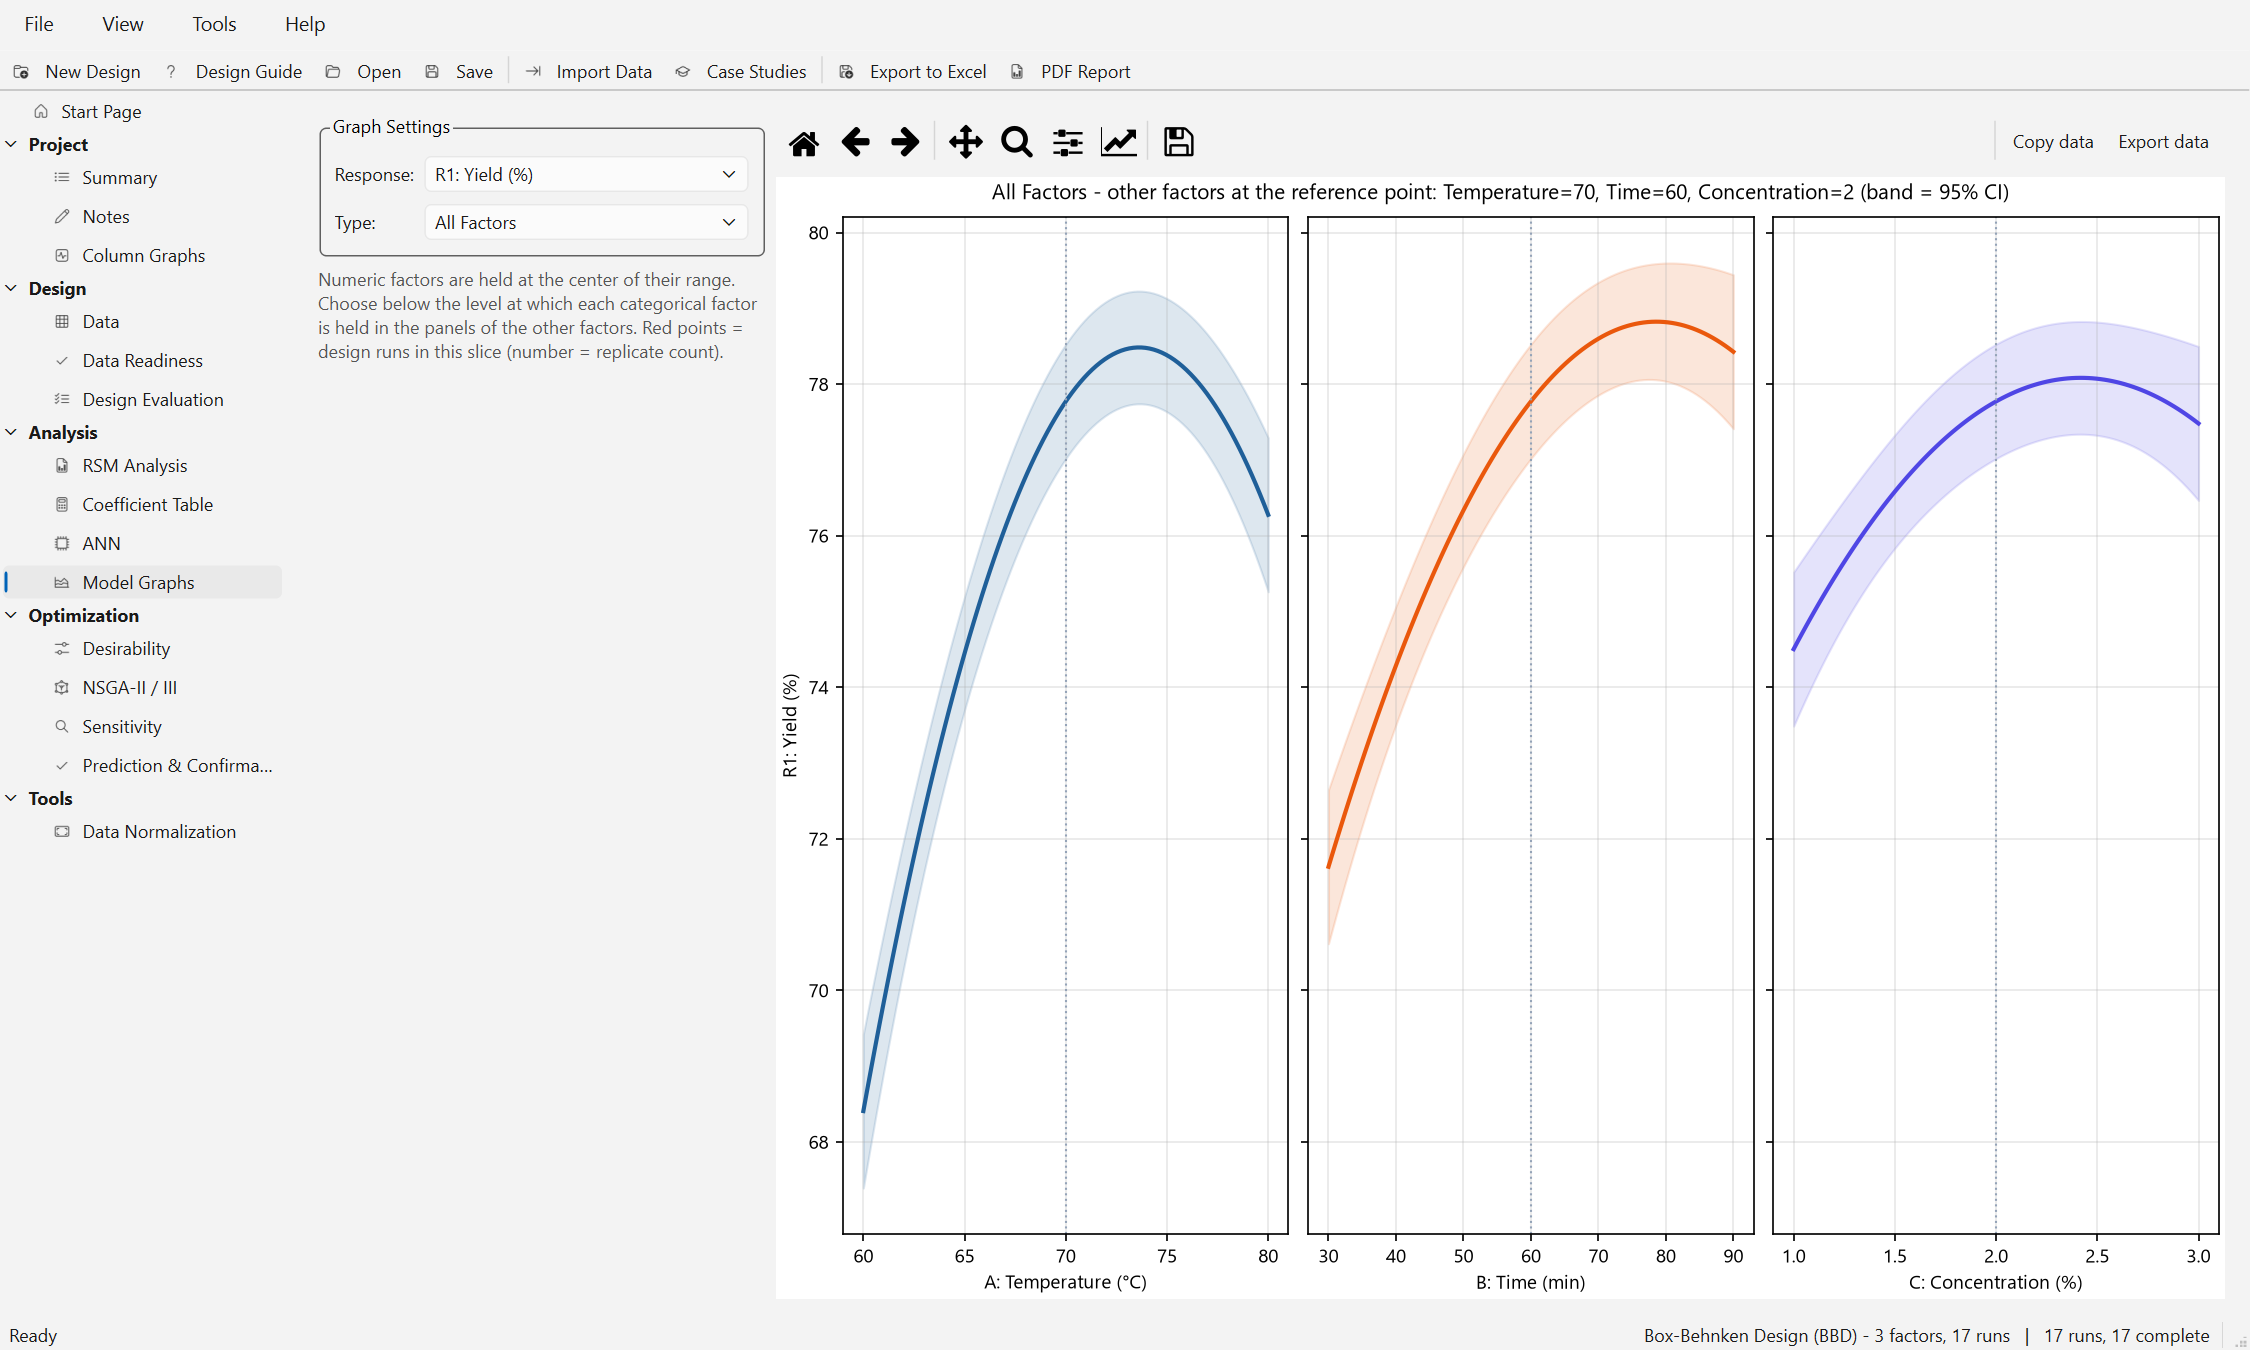
\includegraphics[width=\linewidth]{graph_all_factors.png}
\caption{All Factors graph for Yield: one panel per factor, other factors at the center.}
\label{fig:ch06-allfactors}
\end{figure}

\subsection{Interaction}\label{sec:ch06-interaction}
\paragraph{Purpose.} Shows whether the effect of one factor depends on the level of another.
\paragraph{Output.} The response along the \ui{X axis:} factor, with one line per level of the
\ui{Lines (second factor):} factor: for a numeric factor its low ($-1$) and high ($+1$) level, labeled
``Time low (30)'' and ``Time high (90)''; for a categoric factor one line per level. For a numeric X factor,
95\% error bars are drawn at both ends of each line; for a categoric X factor at every level. Title
``Interaction AB''. Note: ``Non-parallel lines = interaction present. Error bars = 95\% CI.''
\paragraph{Example.} In Figure~\ref{fig:ch06-interaction} the Temperature effect is much stronger at high
Time than at low Time, the AB interaction ($\hat\beta_{AB}=2.14$, $p=0.0005$).

\begin{figure}[htbp]\centering
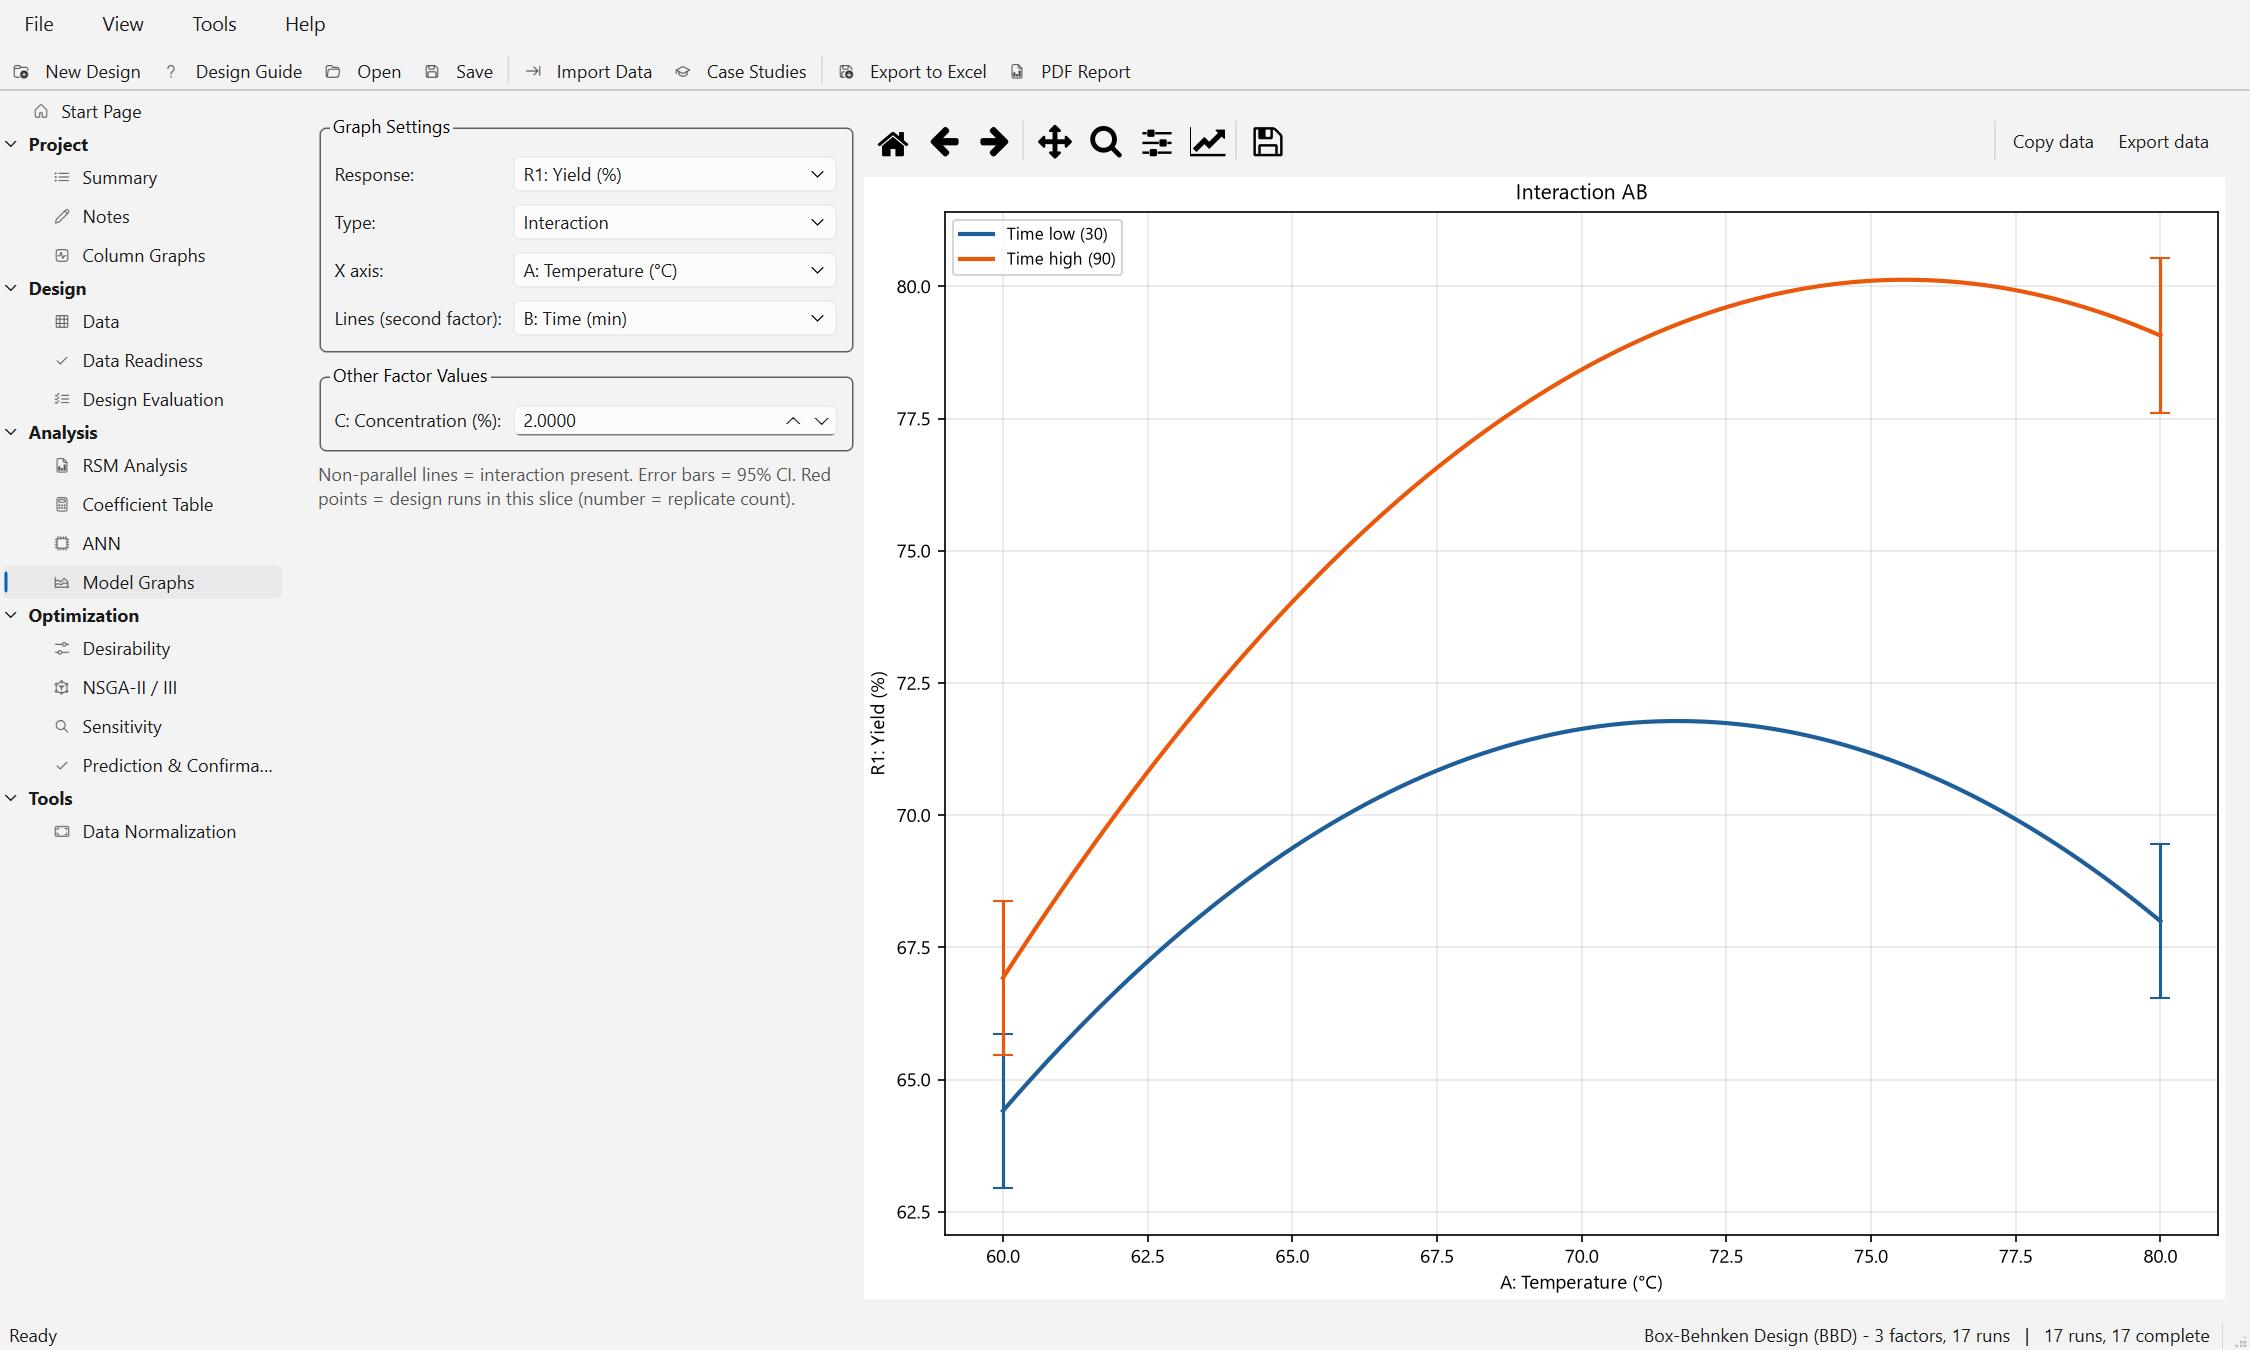
\includegraphics[width=\linewidth]{graph_interaction.png}
\caption{Interaction graph: Yield against Temperature for low and high Time.}
\label{fig:ch06-interaction}
\end{figure}

\subsection{Cube Plot}\label{sec:ch06-cube}
\paragraph{Purpose.} Predictions at the eight corners of three numeric factors, typical for two-level
factorials.
\paragraph{Output.} A cube in oblique projection; each corner shows the predicted response at the
low/high combination (circles colored by value), with the other factors at the slice values. Axis texts give
``low $\rightarrow$ high'' in actual units. Note: ``Corner numbers = predicted response at each low/high level
combination.'' \ui{Copy data} and \ui{Export data\dots} give the table ``Cube corners'' with the three axis
factors in actual units and the predicted response at each of the eight corners; when the design has more factors,
the title lists the values at which the others are held, for example ``Cube corners (D: Solvent = Ethanol)''.
\paragraph{Example.} Figure~\ref{fig:ch06-cube}: predicted Yield ranges from 60.46 (all factors low) to
78.10 (all high).

\begin{figure}[htbp]\centering
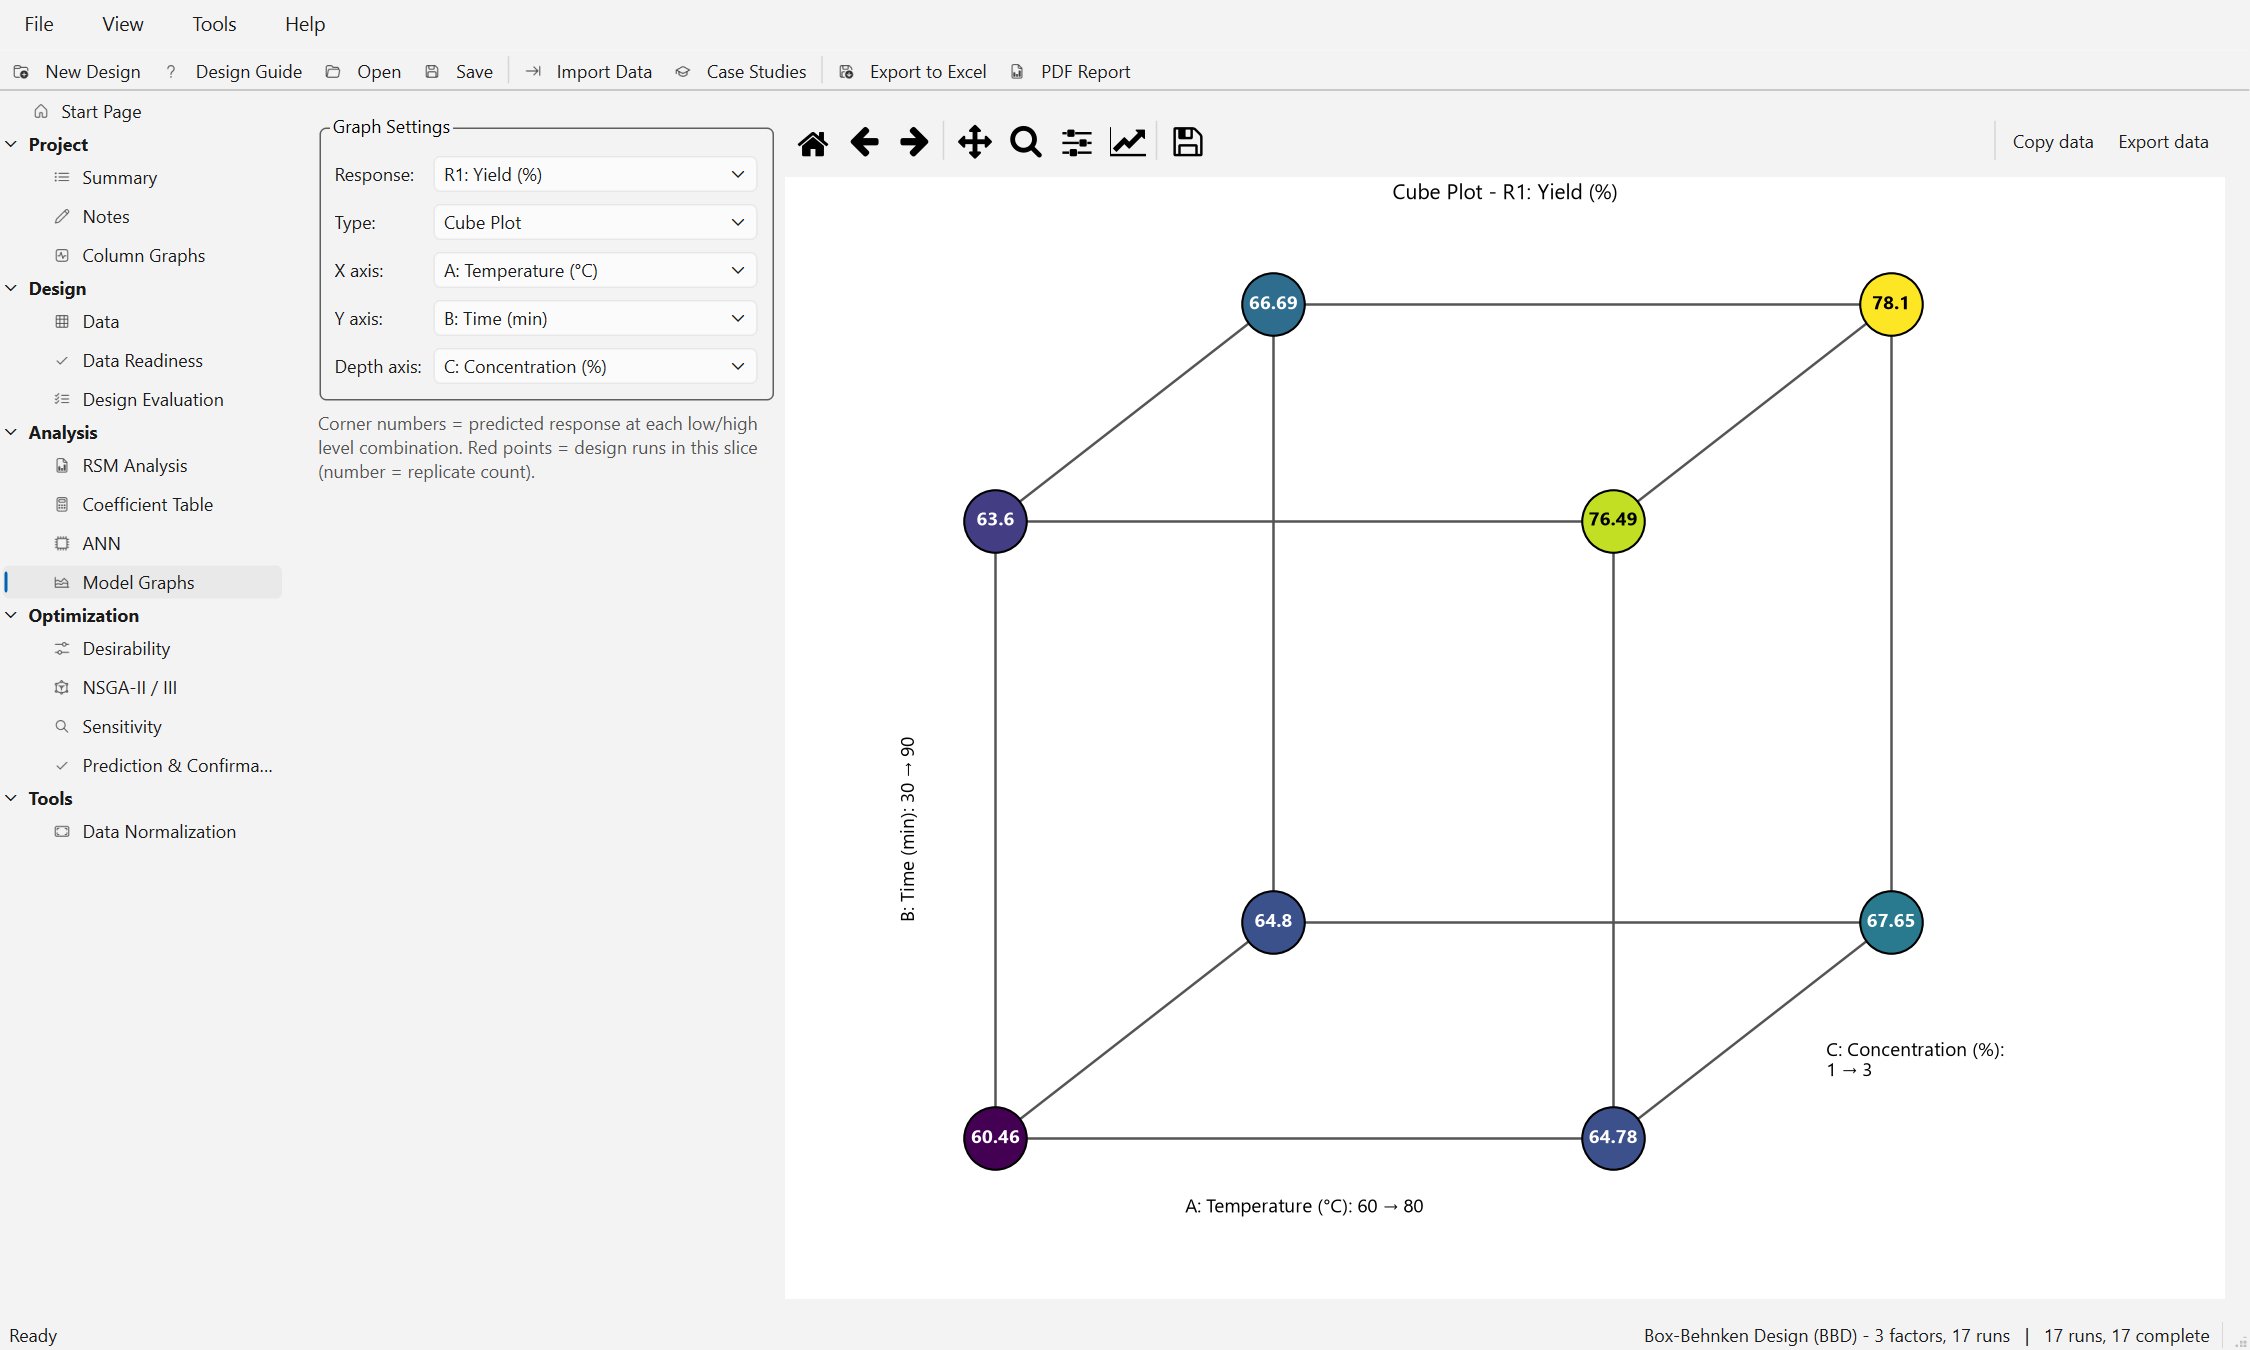
\includegraphics[width=0.85\linewidth]{graph_cube.png}
\caption{Cube Plot of Yield; depth axis Concentration 1 to 3\%.}
\label{fig:ch06-cube}
\end{figure}

\subsection{Perturbation}\label{sec:ch06-perturbation}
\paragraph{Purpose.} Compares all numeric factors around a reference point: a steep trace means a sensitive
factor, a curved trace a quadratic effect, a flat trace an unimportant factor.
\paragraph{How to use.} Set the reference point in the group \ui{Reference Point}, which has a control for
every factor (actual units for numeric factors, a level for categoric factors); it starts at the center of the
ranges.
\paragraph{Output.} Each numeric factor is moved over its whole range, from $-1$ to $+1$ coded units (81
points), while all other factors stay at the reference point, so every trace passes through the reference point.
The x-axis is ``Deviation from reference point (coded units)'': the coded value minus the reference value of that
factor, so a trace runs from $-1-x_{0,i}$ to $1-x_{0,i}$ and covers the full $-1$ to $+1$ span only when the
reference is the center. The title lists the reference values and each trace is labeled with its factor letter.
Note: ``Each numeric factor is moved over its range (-1 to +1) while the other factors stay at the reference point
set below; the x axis is the deviation from the reference value in coded units.'' Not offered for mixture designs
(use the trace plot).
\paragraph{Example.} Figure~\ref{fig:ch06-perturbation}, reference (70 °C, 60 min, 2\%, the center): all
three traces meet at the predicted Yield of the center (77.77); Temperature (A) has the steepest and most curved
trace, Concentration (C) the flattest.

\begin{figure}[htbp]\centering
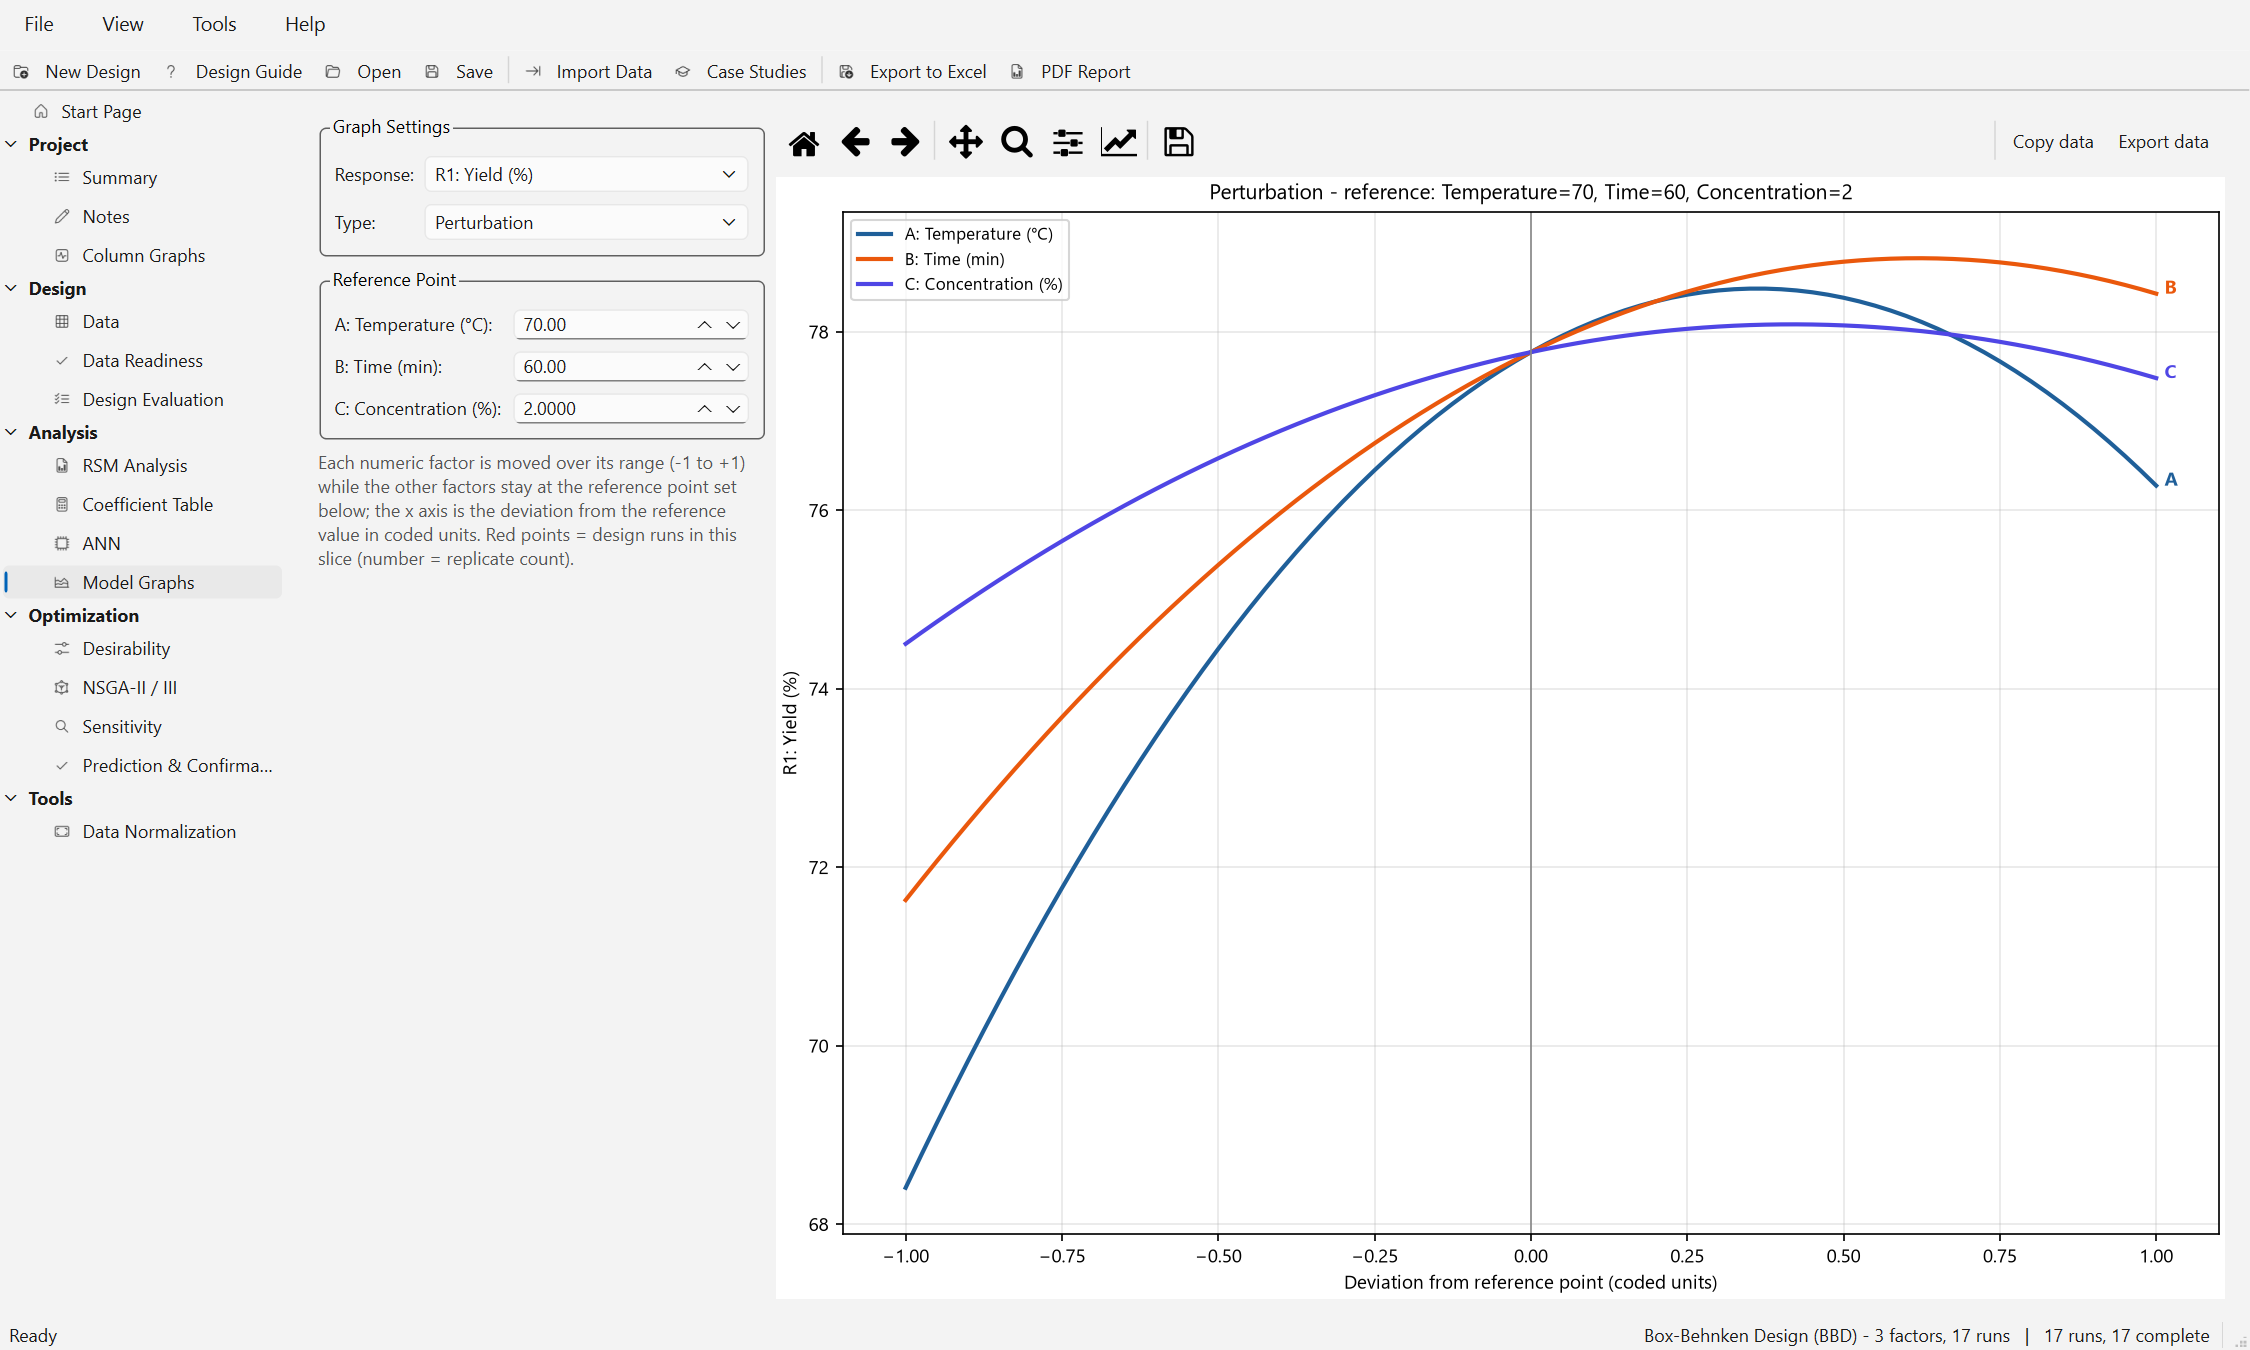
\includegraphics[width=\linewidth]{graph_perturbation.png}
\caption{Perturbation graph for Yield with the \ui{Reference Point} group set to the center of the design
(Temperature 70~°C, Time 60~min, Concentration 2\%).}
\label{fig:ch06-perturbation}
\end{figure}

\subsection{Overlay (Graphical Optimization)}\label{sec:ch06-overlay}
\paragraph{Purpose.} Shows where all responses meet their limits at the same time (the ``sweet spot'').
\paragraph{How to use.} On the \ui{Desirability} page give each response a goal and its \ui{Lower Limit} and
\ui{Upper Limit}. Every response with a goal other than none is used, with the model selected for it.
\paragraph{Theory.} A grid point is acceptable when $L_j\le\hat y_j\le H_j$ for every such response $j$; the
acceptable area is yellow, the rest light grey, and points outside the bounds or constraints darker grey.
Each limit that falls inside the plotted range is drawn as a contour line labeled ``name: value''. Title
``Overlay Plot - yellow = meets all criteria'', with ``(NONE)'' added when no point of the slice qualifies.
Note: ``Each response's limits are taken from the Desirability page (Lower \& Upper Limit for responses with
a goal selected). Yellow area = all responses meet their limits.''
\paragraph{Example.} Figure~\ref{fig:ch06-overlay} uses Yield 75 to 78.29 and Purity 89 to 93.6. With the
goal \emph{maximize}, the upper limit of Yield is the largest observed value (78.29), so the area where the
model predicts more than 78.29 is excluded: it appears as a hole inside the yellow band. Raise the upper
limit if higher values are welcome.

\begin{figure}[htbp]\centering
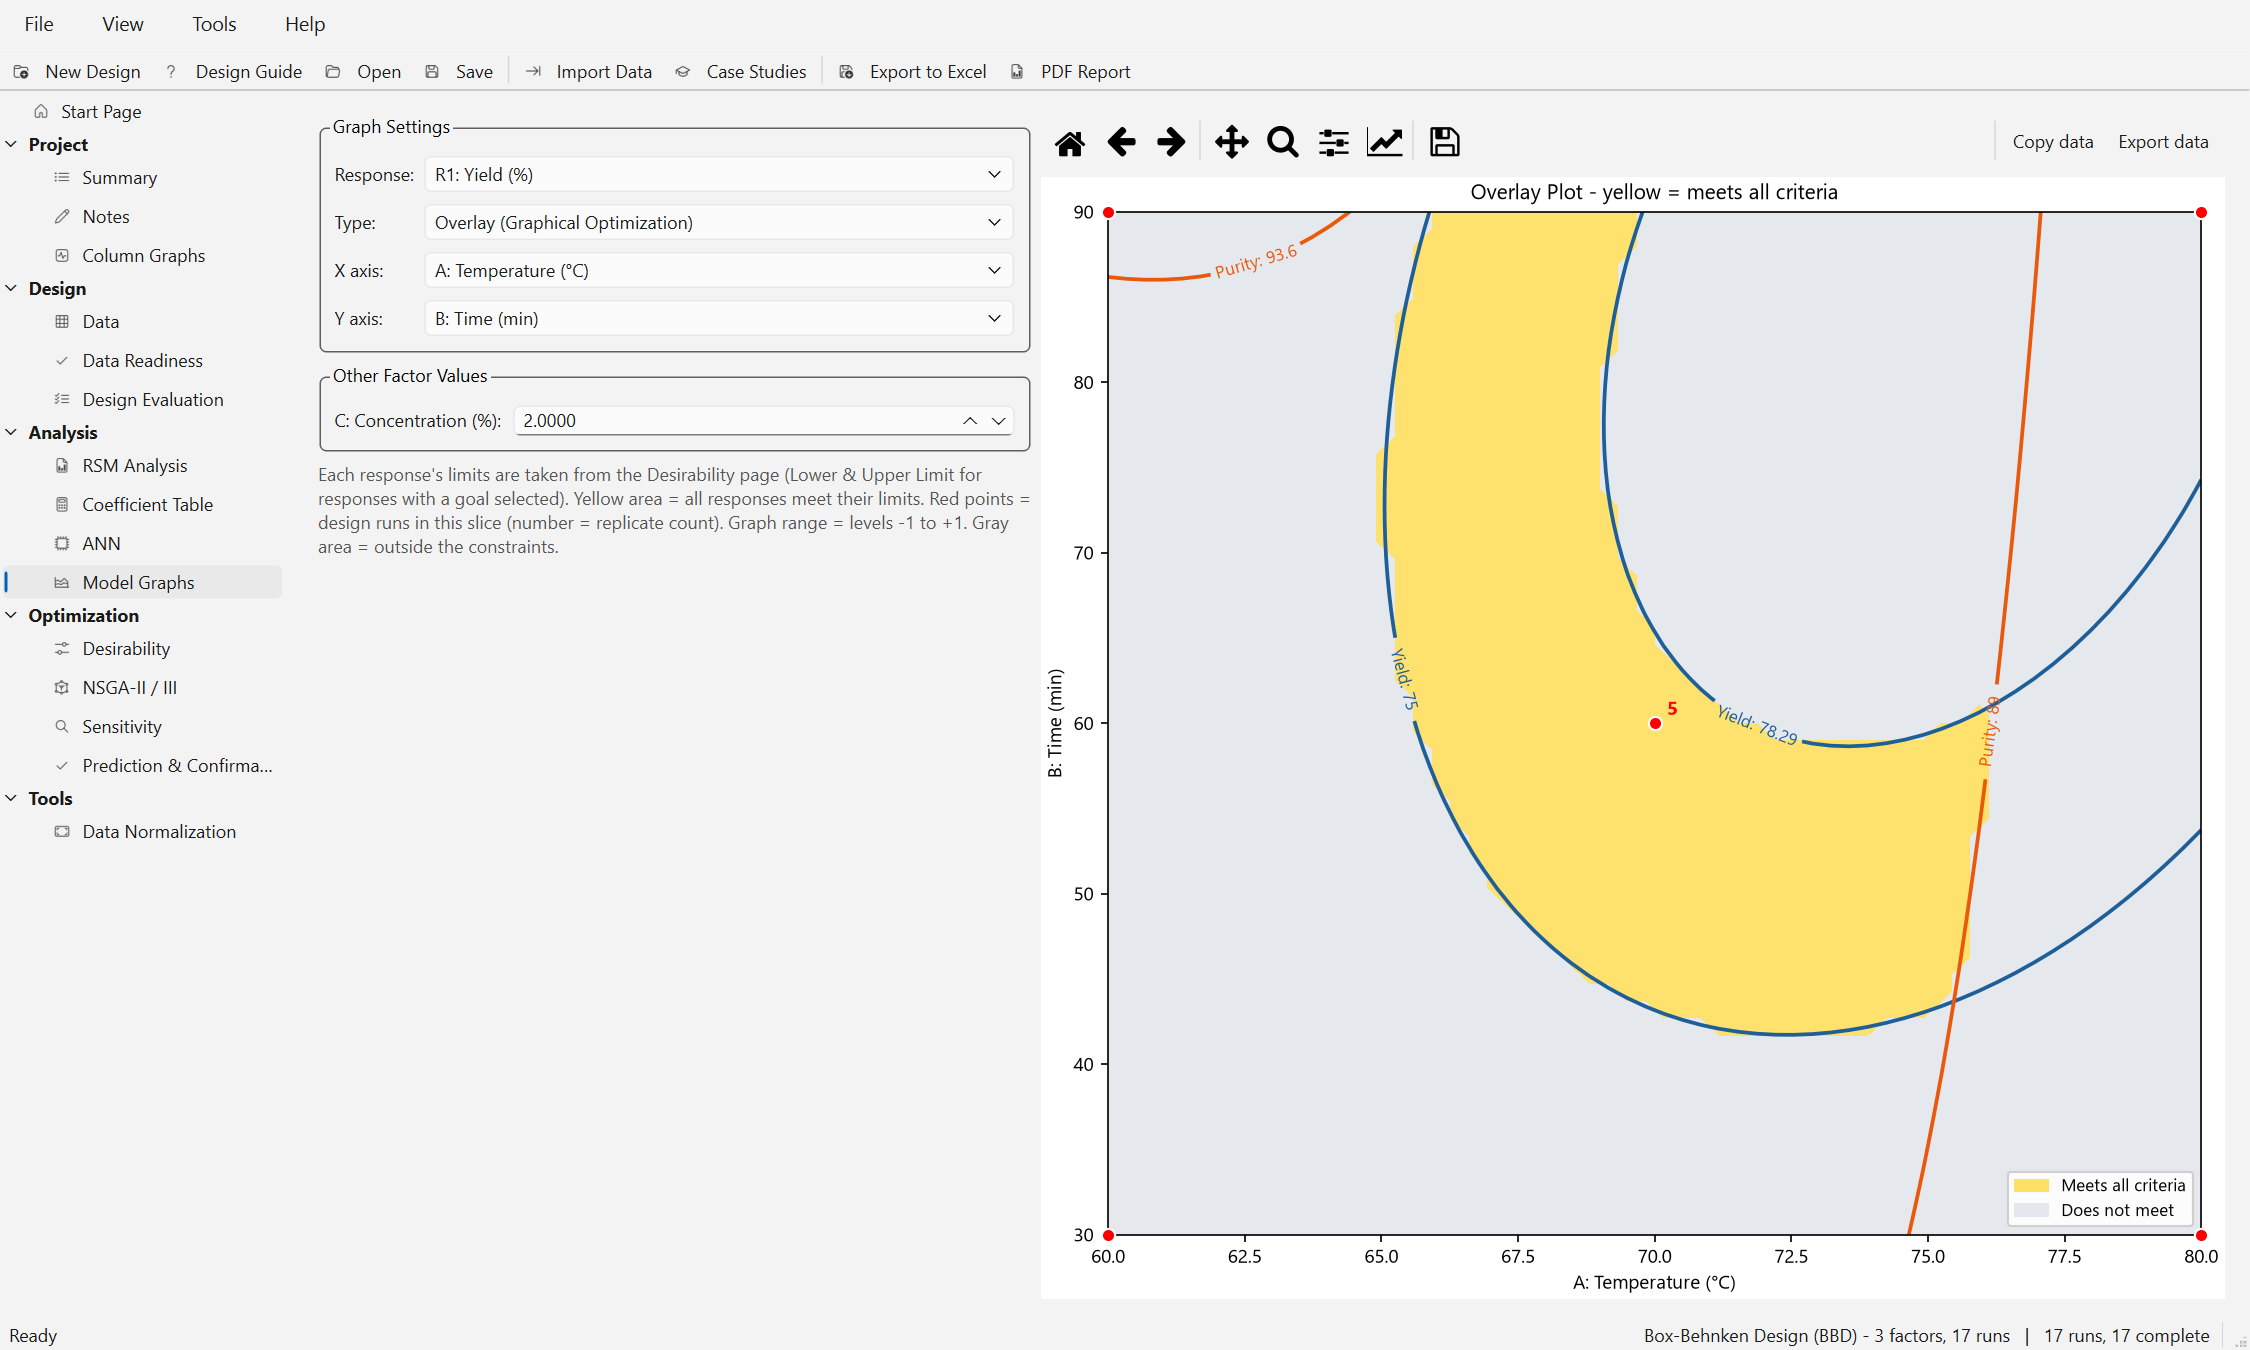
\includegraphics[width=\linewidth]{graph_overlay.png}
\caption{Overlay plot of Yield and Purity; yellow = both responses within their limits.}
\label{fig:ch06-overlay}
\end{figure}

\subsection{Desirability Contour}\label{sec:ch06-desirability}
\paragraph{Purpose.} Shows the combined desirability $D$ of the optimization criteria over the slice, so you
can see how large and how flat the good region is around the numerical optimum.
\paragraph{Theory.} For each response with a goal, the individual desirability \citep{derringer1980} is, with
lower limit $L$, upper limit $H$, target $T$ and shape exponent $s$ (default 1, set on the
\ui{Desirability} page):
\begin{align}
  \text{maximize: }& d=\Big[\text{clip}_{[0,1]}\frac{\hat y-L}{H-L}\Big]^{s},\qquad
  \text{minimize: } d=\Big[\text{clip}_{[0,1]}\frac{H-\hat y}{H-L}\Big]^{s}, \label{eq:ch06-dmax}\\
  \text{target: }& d=\Big(\frac{\hat y-L}{T-L}\Big)^{s}\ (L\le\hat y\le T),\quad
  d=\Big(\frac{H-\hat y}{H-T}\Big)^{s}\ (T<\hat y\le H),\quad d=0\ \text{otherwise}, \label{eq:ch06-dtarget}
\end{align}
and $d=1$ inside $[L,H]$, 0 outside for \emph{In range}. The target defaults to the middle of the limits.
The overall desirability is the importance-weighted geometric mean
\begin{equation}
  D=\exp\Big(\frac{\sum_j r_j\ln d_j}{\sum_j r_j}\Big),\qquad D=0\ \text{if any } d_j=0,
  \label{eq:ch06-D}
\end{equation}
with importance $r_j$ from 1 to 5 (default 3).
\paragraph{Output.} Filled contours of $D$ from 0 to 1 (red to green) with \ui{Contour lines:} levels,
labeled lines, the design points and the optimum star. Note: ``Combined desirability from the criteria on
the Desirability page. Star = latest best solution (if it lies in this slice).''
\paragraph{Example.} In Figure~\ref{fig:ch06-desirability} the best region lies at high Time and
Temperature about 69--72 °C ($D$ up to about 0.83 in this slice). The star is not drawn because the best
solution has Concentration 1.7975\%, not the 2\% of the slice; set Concentration to 1.7975 to see it.

\begin{figure}[htbp]\centering
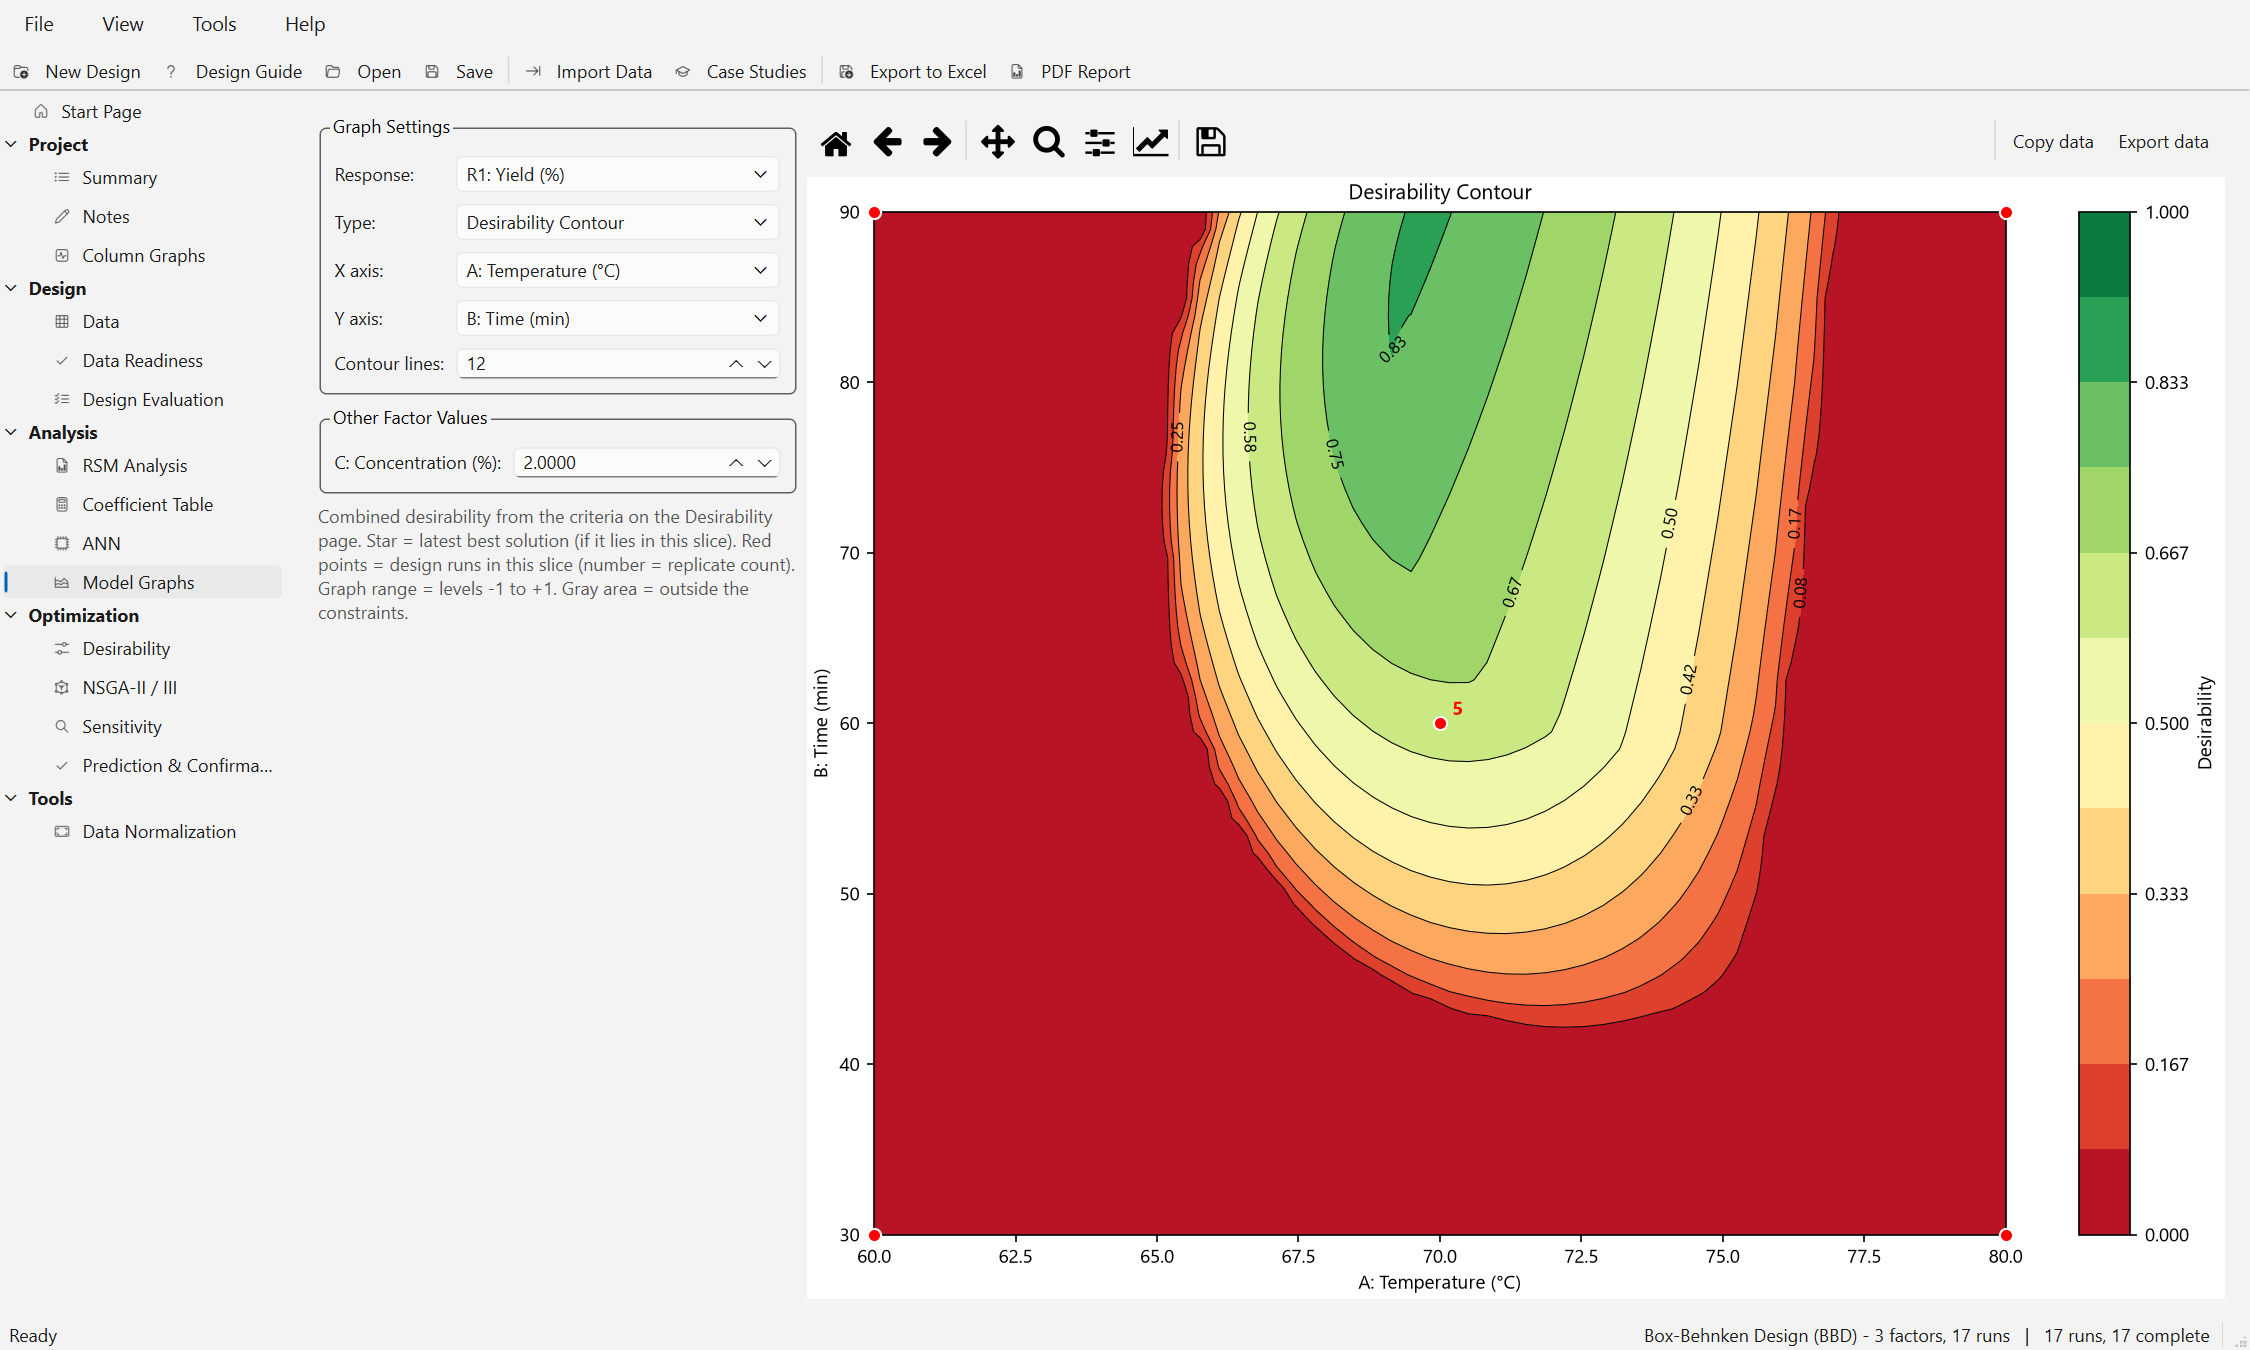
\includegraphics[width=\linewidth]{graph_desirability.png}
\caption{Desirability contour of Yield and Purity (Temperature $\times$ Time, Concentration 2\%).}
\label{fig:ch06-desirability}
\end{figure}

\subsection{Ternary Contour and 3D Ternary Surface}\label{sec:ch06-ternary}
\paragraph{Purpose.} For mixtures the factor space is a simplex; ternary graphs show the response over three
components whose sum is fixed.
\paragraph{How to use.} Choose the components in \ui{Top vertex:}, \ui{Left vertex:} and \ui{Right vertex:}.
With more than three components, or in combined designs, set the other components and the process factors in
\ui{Other Components (Actual Units)}.
\paragraph{Output.} The triangle in pseudo-component space with grid lines for each component labeled in
actual units, filled contours (or a surface), the infeasible area in grey, design points and the optimum
star. Below the triangle: ``Numbers at corners = component amount at the vertex (actual units). Gray area =
outside bounds/constraints.''
\paragraph{Example.} Edible film, Tensile Strength (Figure~\ref{fig:ch06-ternary}): the vertices are Starch
80\%, Glycerol 40\% and Chitosan 40\% (each other component at its lower limit). Strength is highest toward
the Starch-Chitosan edge; the model maximum is about 15.8 MPa at Starch 69.5\%, Glycerol 10\%, Chitosan
20.5\%. Points marked ``2'' are replicated blends.

\begin{figure}[htbp]\centering
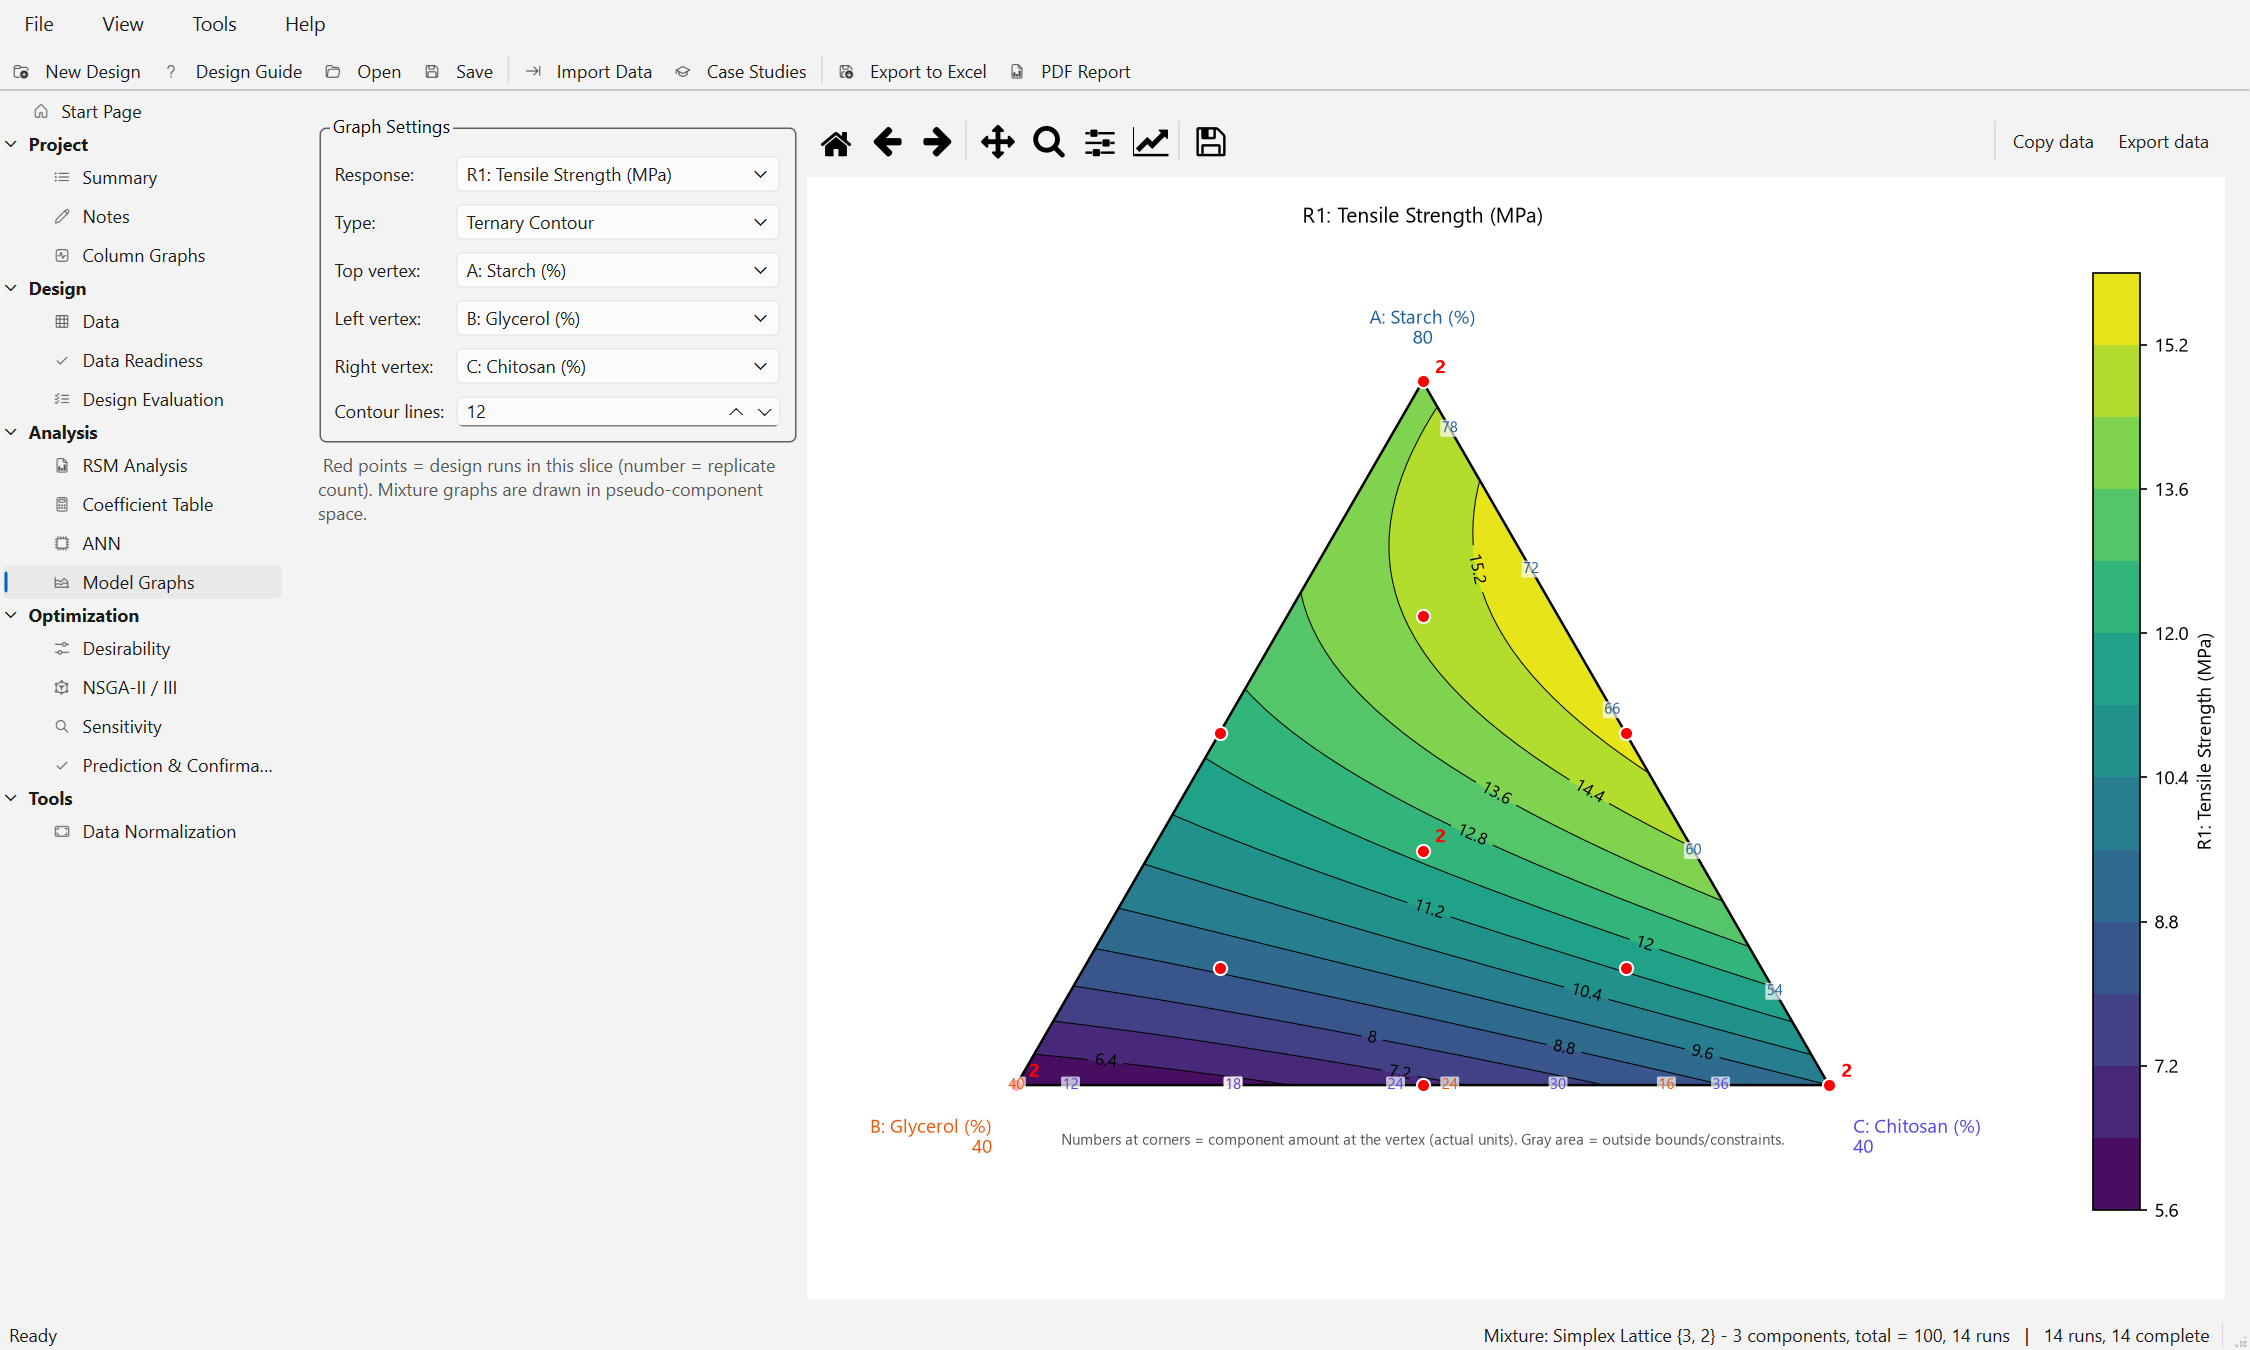
\includegraphics[width=\linewidth]{graph_ternary.png}
\caption{Ternary contour of Tensile Strength (edible film mixture) in pseudo-components.}
\label{fig:ch06-ternary}
\end{figure}

\subsection{Trace (Piepel)}\label{sec:ch06-trace}
\paragraph{Purpose.} The mixture counterpart of the perturbation plot: it shows the effect of each component
when it is increased or decreased from a reference blend while the others keep their relative proportions
\citep{piepel1982,cornell2002}.
\paragraph{Theory.} The reference blend $r$ is the design centroid (mean of the pseudo-component settings).
For component $i$ and $t\in[0,1]$ (201 points)
\begin{equation}
  z_i=t,\qquad z_j=r_j\,\frac{1-t}{1-r_i}\quad(j\neq i),
  \label{eq:ch06-piepel}
\end{equation}
so the sum stays 1 and the ratios between the other components are those of the reference blend
(Piepel's direction). The x-axis is the deviation $t-r_i$ (``Deviation from reference blend
(pseudo-components)''); points outside the bounds or constraints are not drawn. Title ``Trace Plot (Piepel
direction, reference = design centroid)''.
\paragraph{Example.} Edible film, Tensile Strength (Figure~\ref{fig:ch06-trace}), reference blend 60/20/20\%:
increasing Starch raises the strength from 12.2 MPa at the centroid to a maximum of 14.7 MPa at a deviation
of about +0.44; Glycerol lowers it steadily (5.6 MPa at the Glycerol vertex); Chitosan has little effect at
first and lowers it at high amounts.

\begin{figure}[htbp]\centering
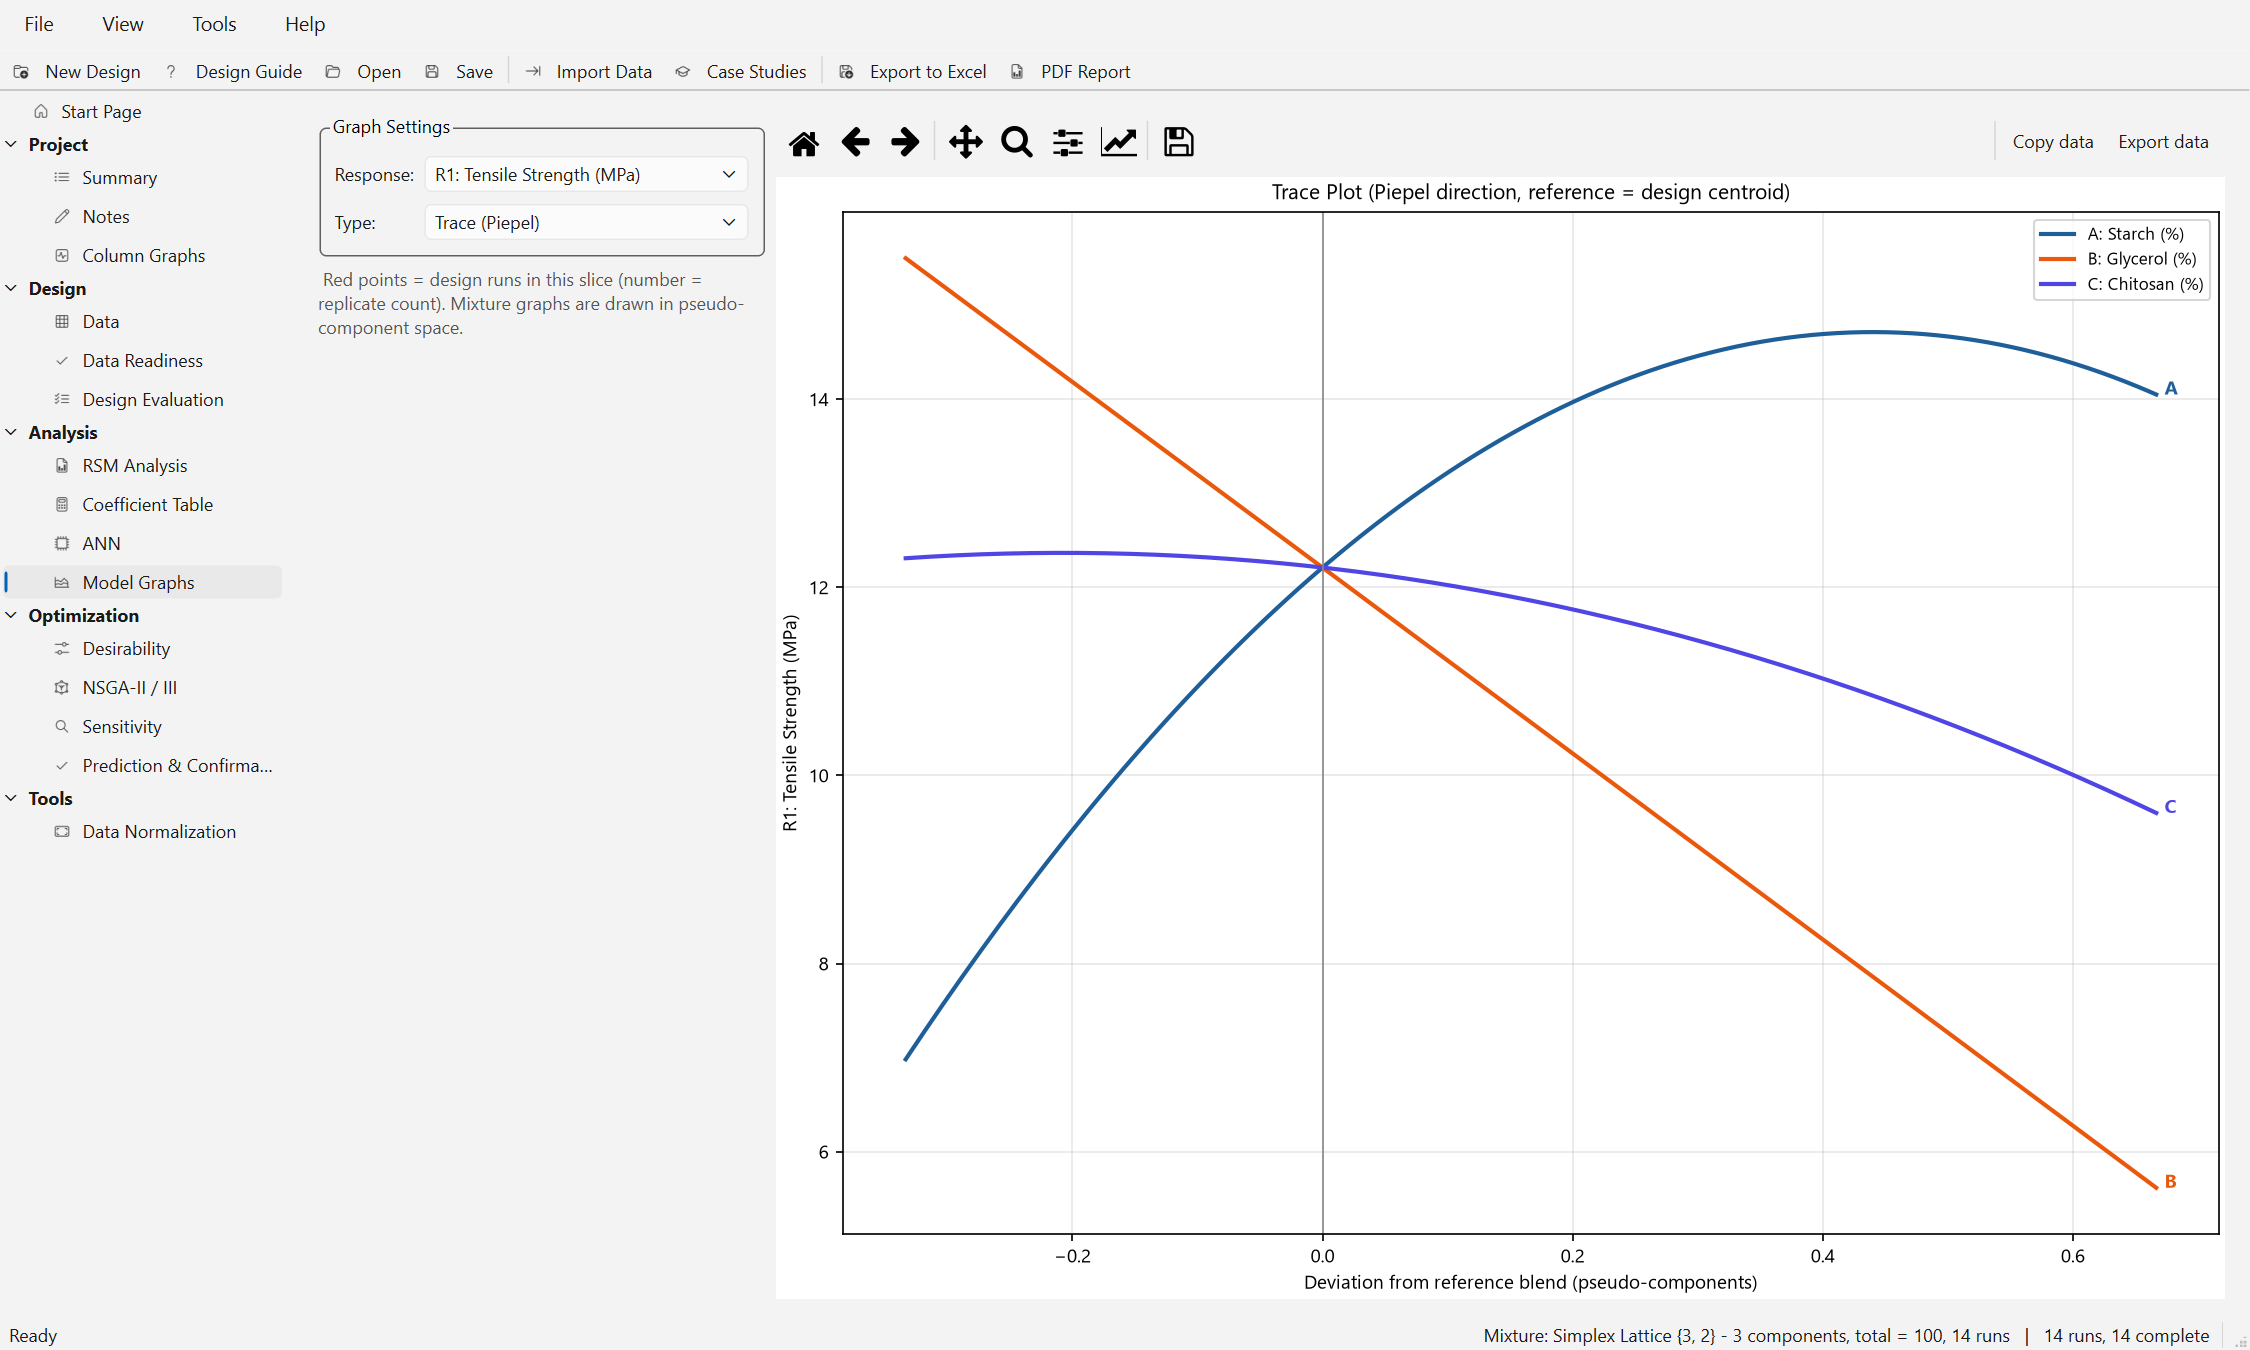
\includegraphics[width=\linewidth]{graph_trace.png}
\caption{Trace plot of Tensile Strength in Piepel's direction from the design centroid.}
\label{fig:ch06-trace}
\end{figure}

\subsection{Propagation of Error (POE)}\label{sec:ch06-poe}
\paragraph{Purpose.} Factors cannot be set exactly in production. POE shows how much variation of the
response is transmitted from the variation of the factors; a robust operating point lies where POE is small.
\paragraph{How to use.} On the \ui{Data} page open \ui{Factor \& Response Info\dots} and enter the standard
deviation $\sigma$ of each factor in actual units (leave it blank for none; not available for categoric
factors). The type \ui{Propagation of Error (POE)} then appears in the \ui{Type:} list. If it is selected
without any $\sigma$, the message ``Enter the factor standard deviations first (Data page $\rightarrow$
Factor \& Response Info...).'' is shown.
\paragraph{Theory as implemented.} With $\sigma_{z,i}$ the standard deviation in coded units
($\sigma_i/h_i$ for a process factor, $\sigma_i/(T-\sum L_j)$ for a mixture component),
\begin{equation}
  \text{POE}(x)=\sqrt{\sum_i\Big(\frac{\partial\hat y}{\partial z_i}\Big)^2\sigma_{z,i}^2
  +\Big(\frac{dg^{-1}(\eta)}{d\eta}\Big)^2\sigma^2_{\text{res}}},
  \label{eq:ch06-poe}
\end{equation}
where the derivatives of the prediction (original units) are central differences with step $10^{-4}$ in
coded units, $g^{-1}$ is the inverse response transformation (its derivative is 1 without a
transformation) and $\sigma^2_{\text{res}}$ is the residual variance: MSE for least squares,
$\hat\sigma^2+\hat\sigma^2_{wp}$ for split-plot models, the mean squared error for an ANN and 0 for GLM
responses. The first term is the variation transmitted by the factors (first-order Taylor expansion, factor
errors assumed independent); the second is the variation that remains even when the factors are set exactly,
so POE is never below $\sigma_{\text{res}}$ for an untransformed response. Mixture components are perturbed
one at a time without renormalizing the blend. The POE graph is a contour plot like
Section~\ref{sec:ch06-contour}, with the title listing the $\sigma$ values.
\paragraph{Example.} Box-Behnken case with $\sigma$ = 1.0 °C, 2.0 min and 0.05\% (Figure~\ref{fig:ch06-poe});
in coded units 0.10, 0.067 and 0.05. In the slice at 2\% Concentration POE ranges from 0.72 to 1.86\%; it is
0.85 at the center. The smallest value, 0.72, lies at about 75 °C and 85 min, close to
$\sqrt{\text{MSE}}=0.714$: there the slope of the surface is almost zero, because this point is the
maximum of Yield in the slice. Here the most productive and the most robust settings coincide.

\begin{figure}[htbp]\centering
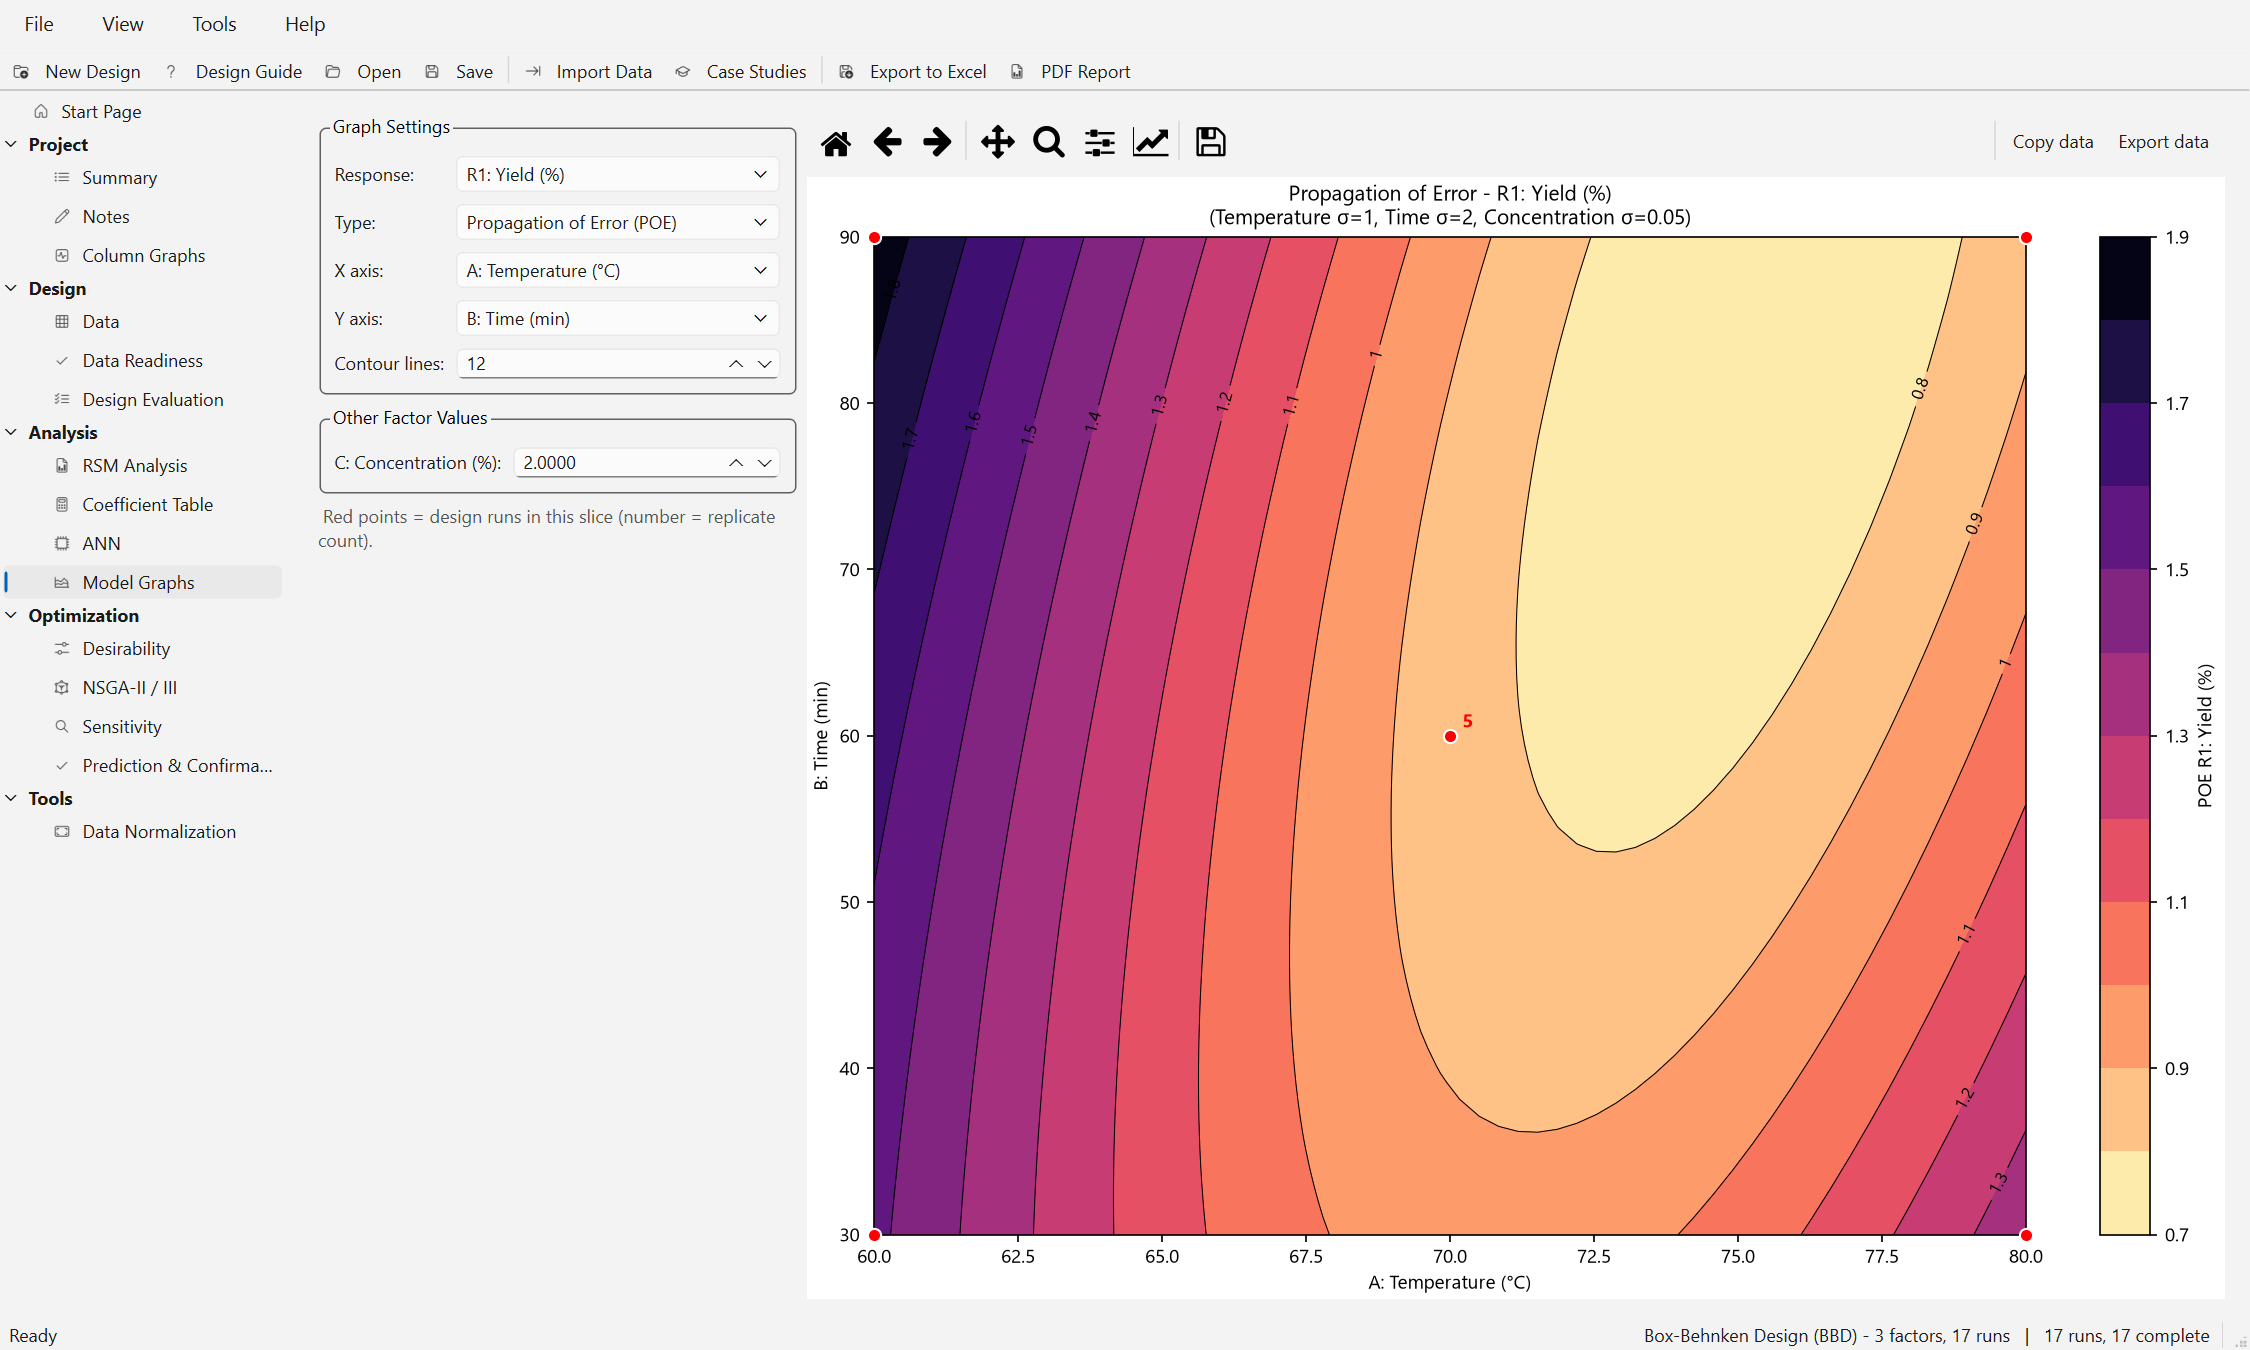
\includegraphics[width=\linewidth]{graph_poe.png}
\caption{Propagation of error of Yield for factor standard deviations of 1.0 °C, 2.0 min and 0.05\%.}
\label{fig:ch06-poe}
\end{figure}

\section{Exporting the data behind a graph}\label{sec:ch06-export}

Every graph can be saved as an image with the toolbar button for saving, and the data behind it can be
reused elsewhere (Figure~\ref{fig:ch06-toolbar}):
\begin{itemize}
  \item \ui{Copy data} (toolbar) or \ui{Copy plot data} (right-click on the plot) puts the data on the
        clipboard, ready to paste into a spreadsheet;
  \item \ui{Export data\dots} (toolbar) or \ui{Export plot data\dots} (right-click) writes an Excel
        workbook with one sheet per data series, or a CSV file with the tables below each other.
\end{itemize}

\begin{figure}[htbp]\centering
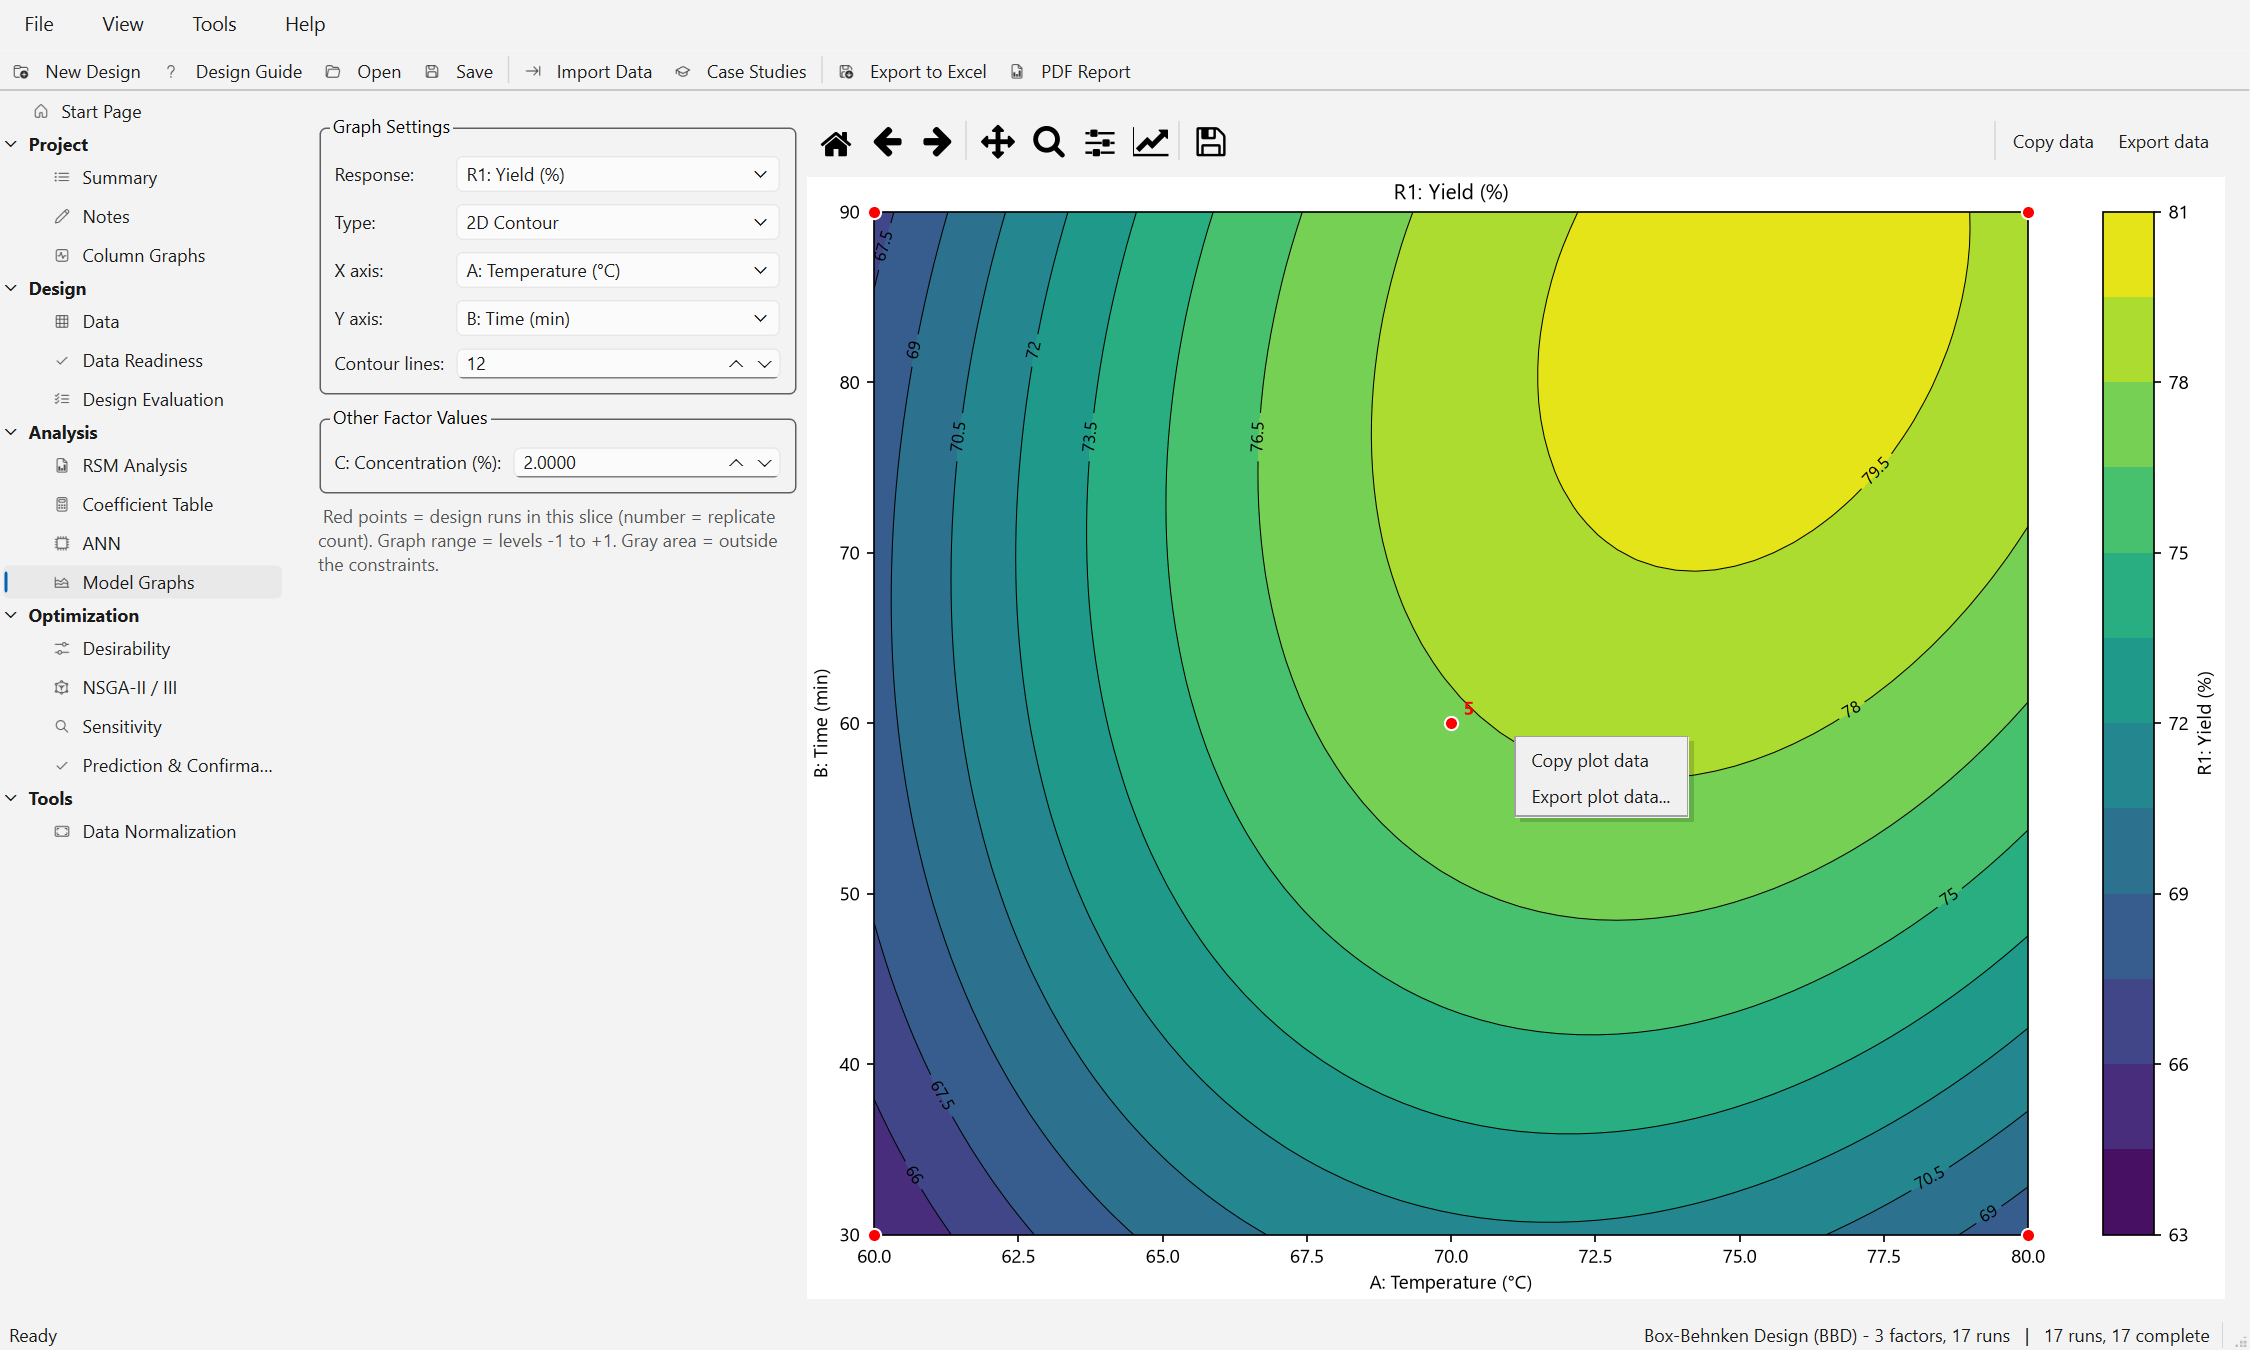
\includegraphics[width=0.75\linewidth]{plot_context_menu.png}
\caption{Right-click menu of a graph with \ui{Copy plot data} and \ui{Export plot data\dots}.}
\label{fig:ch06-toolbar}
\end{figure}

What is exported depends on the graph:
\begin{itemize}
  \item \emph{2D Contour, 3D Surface, ternary graphs, POE}: the full grid. One row per grid point with the
        axis factors in actual units, the column \ui{Inside region (1 = yes)} and the plotted value (the
        response, or \ui{POE} followed by the response name). The table title lists the values of the other
        factors of the slice.
  \item \emph{Overlay}: the grid with the predicted value of each response (column name with its limits)
        and \ui{Meets all criteria (1 = yes)}.
  \item \emph{Desirability Contour}: the grid with the column \ui{Desirability}.
  \item \emph{Design points}: a table ``Design points in this slice'' with the factor values and
        \ui{Number of runs} (3D surfaces: the observed responses); the optimum star, when drawn, as its own
        table.
  \item \emph{One Factor Effect, All Factors}: the predicted line and the 95\% confidence interval
        (columns \ui{Lower} and \ui{Upper}); for categoric factors the points with their error bars.
  \item \emph{Interaction, Perturbation, Trace}: the plotted lines and error bars as drawn.
  \item \emph{Cube Plot}: the table ``Cube corners'' with the eight corners in actual units and the
        predicted response at each corner (the title lists the values of the other factors, if any).
\end{itemize}
To redraw a contour plot in another program, use the grid table, keep the rows with
\ui{Inside region (1 = yes)} equal to 1 and reshape the values to the $60\times60$ grid (process designs).
